\mysection{The simulation}

The simulation built in this work to study the phenomenon of Jet Quenching is performed by coupling JEWEL with an alternative. A description of the models used in this work can be found in Chapter \ref{theory}. First, a simulation was performed with the JEWEL using the default settings, which simulates an idealized version of the initial conditions and the medium\footnote{see Subsection \ref{glauber}}, with the density decaying due to longitudinal expansion only\footnote{see Subsection \ref{bjorken}}. After that, JEWEL code for the medium was modified with an implementation to read the temperature profiles of an arbitrary model. This allowed us to study the effects of different initial conditions and also a realistic hydrodynamic evolution. For this, a choice was made to create a grid with spacing $0.15 \,\rm fm$ on which the temperature profile was read from a foreign model. The time step used is of $0.1 \,\rm fm/c$. This is a time step larger than necessary for hydro simulations, but we are not integrating differential equations, so this does not insert great numerical errors, for more detail refer to the discussion on the last session of this chapter. For intermediate values, a bicubic interpolation was used.
\par 
After this procedure, the generated events on JEWEL were passed on to Rivet\cite{bierlich_robust_2019} for analysis. Rivet is a package for analysis of the generated Monte-Carlo events. It also makes use of the FastJet\cite{cacciari_fastjet_2012} package. The observables generated were the ones in Section \ref{algorithms}. The uncertainty on the histogram bins presented in Sections \ref{jewel_with_ic} and \ref{jewel_with_hydro} are calculated for a binomial distribution according to the statistics generated by the Monte-Carlo events.
\par
The simulation in each of the cases consists of a thousand of different medium profiles, and ten thousand JEWEL Monte-Carlo events generated for each profile. The different simulated scenarios are displayed in Table \ref{scenarios}. The analysis was performed in the $0-10\%$ centrality class for $\sqrt{s_{NN}} = 2.76 \, {\rm TeV}$ collision energy. The Rivet package was then used for the analysis of the Monte-Carlo events. In the case of charged jet observables, scaling factors were extracted from proton-proton collisions, both on the jet energy and also on spectrum normalization\cite{zapp_geometrical_2014}. These factors allow us to compare the analysis of full jets and charged jets. We extract them by matching the spectra of a given observable in pp collisions by scaling it. It is then assumed that the factors are the same in heavy-ion collisions. An example is the jet $p_T$, in this case, since charged jets have fewer particles, its momentum will be smaller, and scaling for comparison is necessary. A factor of $3/2$ was obtained in \cite{zapp_geometrical_2014}.

\begin{table}
\centering
\begin{tabular}{| c | c | c |}
 \hline 
 \multicolumn{3}{| c |}{Scenarios} \\
 \hline
 \hline
            & Initial conditions & Evolution \\ 
 \hline
 Default              & Ideal   & \multirow{3}{10em}{Longitudinal expansion} \\ 
 \cline{1-2}
 \trento              & \trento & \\
 \cline{1-2}
 MC-KLN              & MC-KLN & \\
 \hline
 v-USPhydro + MC-KLN  & MC-KLN  & 2+1 v-USPhydro code \\
 \cline{1-2}
 \hline
\end{tabular}
\caption{Scenarios simulated in this work. See Charter \ref{theory} for explanation on the items of the table.}
\label{scenarios}
\end{table}

To include the new medium profile in JEWEL, a choice was made to build a grid with local values of the temperature. The spacing of the grid is about $0.15 \, {\rm fm}$. The time-step was taken to be $0.1 \, {\rm fm/c}$. The information was then passed to JEWEL upon request through a function $T(x,y,\tau)$. The $\tau$ coordinate is the proper-time and the $x$ and $y$ coordinates are the transverse coordinates, relative to the beam axis. $\tau$ was taken to be equal $\sqrt{t^2-z^2}$ according to a boost invariance assumption. If one chooses not to make this assumption, a 3+1 code simulation for the hydrodynamics is necessary. The restriction to mid-rapidity of all analysis was then used. For values outside the gridpoints, a bicubic interpolation was used\cite{vetterling_numerical_1992}, and on the proper-time coordinate, a linear interpolation was used.
\par
Since only a temperature profile was provided to JEWEL, a choice of an EOS had to be used to provide a density of scattering centers profile. This was used through an ideal equation of state. This equation of state was taken as $n \propto T^4$. This is the dependence as one would have for the formalism described in Section \ref{qgp}. Also, no local fluid velocity was assumed. Any momentum that the scattering centers might have comes from a kinetical description.

\mysection{Jet Algorithms}
\label{algorithms}

Jets are a consequence of the confinement property of strong interactions\cite{halzen_quarks_1984,peskin_introduction_1995,salam_towards_2010}. It happens because, since the partons coming out of a hard scattering are very energetic, their energy must be converted into a multitude of hadrons. One common picture of this is that the field between a parton dipole is seen as a tube connecting them. It is a consequence of the self-interaction of the gluon field that the lines of force do not spread out into space, but are contained in the space between the partons. Once the distance between the partons starts to grow, the energy stored in this flux-tube starts to grow linearly. Eventually, it becomes favorable for the system to exchange a portion of this tube for a pair of partons pulled out of the vacuum, turning it into two pairs of partons with two chromoelectric tubes. The process continues repeatedly until the energy in each pair is no longer enough to break the strings. At this point, these less energetic systems might decay into the known hadron states.
\par
Armed with the qualitative idea of what a jet is, a definition must be made in a more quantitative ground. This definition must account for certain conditions that are defined in the Snowmass accord\cite{salam_towards_2010}:

\begin{itemize}

\item Simple to implement in an experimental analysis;
\item Simple to implement in the theoretical calculation;
\item Defined at any order in perturbation theory;
\item Yields finite cross sections at any order of perturbation theory;
\item Yields a cross-section that is relatively insensitive to hadronization;

\end{itemize}

The difficulties that the previous accord tried to address are related to the fact that jets are ill-defined objects. There is a major uncertainty because jets are a consequence of non-perturbative physics, which is poorly understood. The way one defines a jet, then, is by defining an algorithm that clusters particles into jets. With this algorithm, experimental analysis can be performed. On the theory side, one usually implements a model for fragmentation and hadronization and later applies the jet algorithm to the final state to make comparisons with data. There is also the alternative to invoke parton-hadron duality and claim the jet 4-momenta are directly comparable to partons momenta\cite{dissertori_quantum_2003}.
\par
Building an algorithm might have some difficulties due to infinities that appear in calculations at the theoretical level. Some of these infinities might be washed away from the calculations by grouping different final states together. The problem, then, is that the algorithm must treat these final states on the same ground as well.
\par
One of these situations arises when a parton splits collinearly. This situation is illustrated in Figure \ref{collinear_safe}. The loop diagram for the case that the partons merge again cancels its divergence with the case in which the partons split and do not merge. This means that, at the theoretical level, the two cases must be treated at the same level. In Figure, we see the difference between theoretically safe and an unsafe algorithm. An unsafe algorithm might see a hard seed on the high transverse momentum particle on the left and cluster from there. This would result in two jets. A safe algorithm would not be subject to this problem.

\begin{figure}
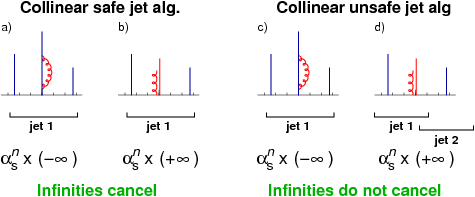
\includegraphics[width=1.0\textwidth]{images/collinear_safe.png}
\caption[Collinear safe ilustration]{A description of collinear safe and an collinear unsafe algorithm. Here we have two situations that must be treated on equal grounds due to theoretical reasons and might not be so due to the choice of jet algorithm. Figure from \cite{salam_towards_2010}}
\label{collinear_safe}
\end{figure}

Another type of problem that might occur is due to soft radiation. This situation can be seen in Figure \ref{infrared_safe}. As before, we have two final states that must be treated on the same ground, from the theoretical perspective. But the algorithm might not do so. It can happen because the extra particle seen in red in the Figure might act as a new seed and cluster two jets into one. Algorithms that succeed in avoiding this merging are called infrared safe.

\begin{figure}
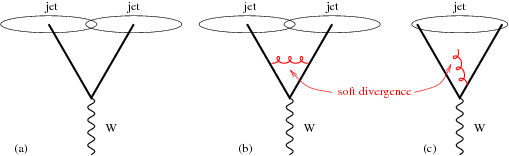
\includegraphics[width=1.0\textwidth]{images/infrared_safe.png}
\caption[Collinear safe ilustration]{A description of infrared safe and an infrared unsafe algorithm. Here we have two situations that must be treated on equal grounds due to theoretical reasons and might not be so due to the choice of jet algorithm. Figure from \cite{salam_towards_2010}}
\label{infrared_safe}
\end{figure}

One of the algorithms that satisfy to a good extent these criteria is the anti-kt algorithm\citep{cacciari_fastjet_2012}. The anti-kt algorithm belongs to a broader class called the recombination algorithms. The members of this class are all based on the idea of a distance defined between every pair of particles being analyzed. If the distance is smaller than the distance of another particle to the beam, the particles are combined. This process is repeated until no single pair satisfies the condition and one ends up with a set of jets of the event. At this stage, further cuts might be done in the rapidity or the $p_t$ of the jet. The distance used in the anti-kt algorithm is defined by the following equation:

\begin{equation} \label{jet_alg}
d_{ij} = \min (p_{t i}^{2p},p_{t j}^{2p}) \frac{\Delta R_{ij}}{R}
\end{equation}

Where $R$ is a parameter that is defined at each analysis. For $p=-1$\footnote{The value $p=1$ corresponds to the $k_t$ algorithm and $p=0$ to the Cambridge-Achen. See \cite{salam_towards_2010} for further details}. Where:

\begin{equation} \label{delta_r}
\Delta R_{ij} = \sqrt{ (\eta_i - \eta_j)^2 + (\phi_i - \phi_j)^2 }
\end{equation}

A distance to the beam axis is also defined:

\begin{equation}
d_i = p_{ti}^{-2}
\end{equation}

From all the $d_{ij}$ and $d_i$ the minimum value is chosen. If it is $d_i$ then this particle is removed from the list and called a jet. Otherwise, it is a distance $d_{ij}$, the $i$ and $j$ particles are combined. The process goes on iteratively until a final list of jet candidates is left. The recombination of the particles is performed using the $E$ scheme, or 4-momentum scheme, which means particles are combined by adding their 4-momenta.

\mysubsection{Background subtraction}

An extra difficulty arises when trying to perform jet analysis in heavy-ion collisions due to the background contamination, called the Underlying Event (UE). The UE corresponds to the soft particles that come from the radiation of the freeze-out surface and are mainly explained through hydrodynamics. When one is trying to cluster jets, experimentally, one must subtract this background in other to make comparisons with theory.
\par
In JEWEL, the recoiling scattering centers can be kept and included in the final state of the events. Whenever there is an elastic collision during the parton propagation, the distinction between the 4 momentum that is part of the jet and the 4 momentum that is part of the medium is spoiled. To address this problem, the scattering centers kept by JEWEL are used to subtract this 4 momenta from the final state.
\par
Following \cite{zapp_geometrical_2014}, the background subtraction is performed by the use of ghost particles. These particles are inserted into the final state with very low $p_T$ and the same direction as the four-momentum assigned to the scattering center. Particles are then classified as background if they satisfy the following condition:

\begin{equation}
\Delta R_{ij} < 1 \cdot 10^{-5}
\end{equation}

Where $\Delta R_{ij}$ is the distance to the closest ghost particle (see Equation \eqref{delta_r}). The list compiled by evaluating this condition is then subtracted according to each observable. In the case of jet girth, for instance, the particles deemed to be background are removed from the jet constituents list and thus do not participate of the observable calculation. In the case of jet dispersion, we used:

\begin{equation}
p_T^D = \frac{\sqrt{ \sum_{\rm particles} {p_t}^2 - \sum_{\rm background} {p_t}^2 }}{p_{t,corrected}^{jet}}
\end{equation}

For the jet mass, a correction of the jet four-momentum comes automatically when removing the background from the list of particles.

\mysection{Jet Observables}

Although the main idea of a jet is to reconstruct the basic partonic kinematics of a hard scattering, there are a lot of things that can be investigated with a jet. This is since the jet has more information than a single particle. One can study its shape and structure to find radiation patterns and non-perturbative dynamics. In the present work, the main idea is to look for radiation patterns. Here we define the observables that can characterize the jets used in this work.

\mysubsection{Girth}

The generalized angularities for the jet constituents are defined as:

\begin{equation} \label{gen_ang}
\lambda_{\beta}^{\kappa} = \sum_i \left( \frac{p_{T,i}}{p_{T,jet}} \right)^\kappa \left( \frac{\Delta R_{jet,i}}{R} \right)^\beta
\end{equation}

Where $\kappa$, $\beta$ and $R$ are parameters chosen at each analysis. $\Delta R_{jet,i}$ is the angular distance between jet and constituent $i$. Girth is related to the angular opening of the jet. The idea is to pick the first order moment in angular distribution with the constituents $p_T$ as weights. This means picking $\beta=\kappa=1$. Girth is defined by:

\begin{equation}
g = \sum_{\rm constituents} \frac{p_t}{p_t^{jet}} \Delta R_{i,jet}
\end{equation}

Where $\Delta R_{i,jet}$ is calculated according to \eqref{delta_r} and the sum is taken on the constituents of the jet. Its possible values lie in the $\left[ 0,1 \right]$ interval. Girth is also known in some collaborations as jet width. Unlike the jet mass, it depends linearly on the transverse momentum of the constituent particles. Therefore, it is more sensitive to softer fragmentation.

\mysubsection{Dispersion}

This observable measures the \emph{hardness} of the fragmentation of the jet. This means that it will have a large value if the jet $p_t$ is distributed in fewer particles, and smaller values if the $p_t$ is distributed in a larger number of particles. Its definition is given by the equation:

\begin{equation}
p_T^D = \frac{\sqrt{ \sum_{\rm constituents} {p_{t,i}}^2 }}{p_t^{jet}}
\end{equation}

Where the sum is taken on the constituents of the jet. It corresponds to $\kappa=2$ and $\beta=0$ in Equation \eqref{gen_ang}. It can be seen from its definition that the possible values lie in the $\left[0 , 1 \right]$ interval. Values close to one will correspond to the extreme case of the jet transverse momentum being distributed in one or two constituents and one of them carries most of its momentum. The opposite limit corresponds to the jet transverse momentum being distributed almost equally on a high number of constituents.

\mysubsection{Jet Mass}

The jet mass is a observable that is constructed from the jet four-momentum in the usual Lorentz formalism. The definition is:

\begin{equation}
M_J = \sqrt{ \left( \sum_{\rm particles} {\rm E} \right)^2 - \left( \sum_{\rm particles} {\rm \overrightarrow{p}} \right)^2 }
\end{equation}

It can be seen, in the RHS of the above equation that this observable is sensitive to the collimation of the jet. This can be observed by noting that, inside the square root, there is a scalar sum and a vector sum, where vector sum depends on the angular separation of the constituents. The broader the jet, the smaller the jet mass. And the impact of each constituent particle in this observable depends on the squared transverse momentum. This increases the impact of the harder constituents of the jet.


%\mysubsection{SoftDrop}

%There is another interesting observable regarding the substructure of a jet that is the fraction of $p_T$ carried by the softest of the two proto-jets forming a jet. To find this quantity, one must first apply the anti-kt algorithm to an event. After that, one runs the C/A algorithm just on the constituents of a given jet until there are two proto-jets. If they satisfy the SoftDrop condition:

%\begin{equation}
%z = \frac{\min (p_T^A, p_T^B)}{p_T^A + p_T^B} \Delta R^{\beta} > z_g
%\end{equation}

%Then $z$ is counted on a histogram, else, the highest $p_T$ jet is inserted back into the C/A and the process is repeated. This observable tries to find the first and hardest splitting that the parton that gave birth to the jet went through.

\mysubsection{Azimuthal anisotropy $v_2$}

The azimuthal anisotropy for a given observable comes from the idea of expanding a given spectrum in the following form:

\begin{equation}
\frac{{\rm dN}}{{\rm d}^2p_T {\rm d}\eta {\rm d}\phi } = \frac{{\rm dN}}{{\rm d}^2p_T {\rm d}\eta } \left[ 1 + \sum_n 2 v_n \cos \left( n ( \phi - \Psi_{\rm RP} ) \right) \right]
\end{equation}

Where $\Psi_{\rm RP}$ is the reaction plane angle. The coefficients $v_n$ are adjusted and represent the lack of cylindrical symmetry of the spectra. $v_2$ is called the azimuthal anisotropy coefficient and $v_3$ is the triangular flow. They usually reflect the geometry of the initial conditions set by the early dynamics, before the hydro phase. The harder problem in the measurement of these quantities is the determination of the reaction plane, which is random. Usually, it is calculated by adjusting the above formula with the distribution in $\phi$ of the observed particles in an event. The $v_2$ coefficient is related to the ellipticity of the initial conditions for the hydro expansion. As can be seen in Figure \ref{v2}, it comes from the shape of the overlap zone of the colliding nuclei.

\mysection{Grid validation}

As a validation for the grid method implemented in this work, we show here a comparison between observables calculated with JEWEL in its default configuration and with the grid method implemented here. In Figure \ref{grid_jetpt_validation} we can see the jet $p_T$ spectrum for both cases. And in Figure \ref{grid_default} we can see a ratio plot of both spectra. Within the statistical uncertainty calculated for the Monte Carlo, we can see that they both agree. This result shows that errors inserted due to interpolation of the grid do not affect this observable.

\begin{figure}
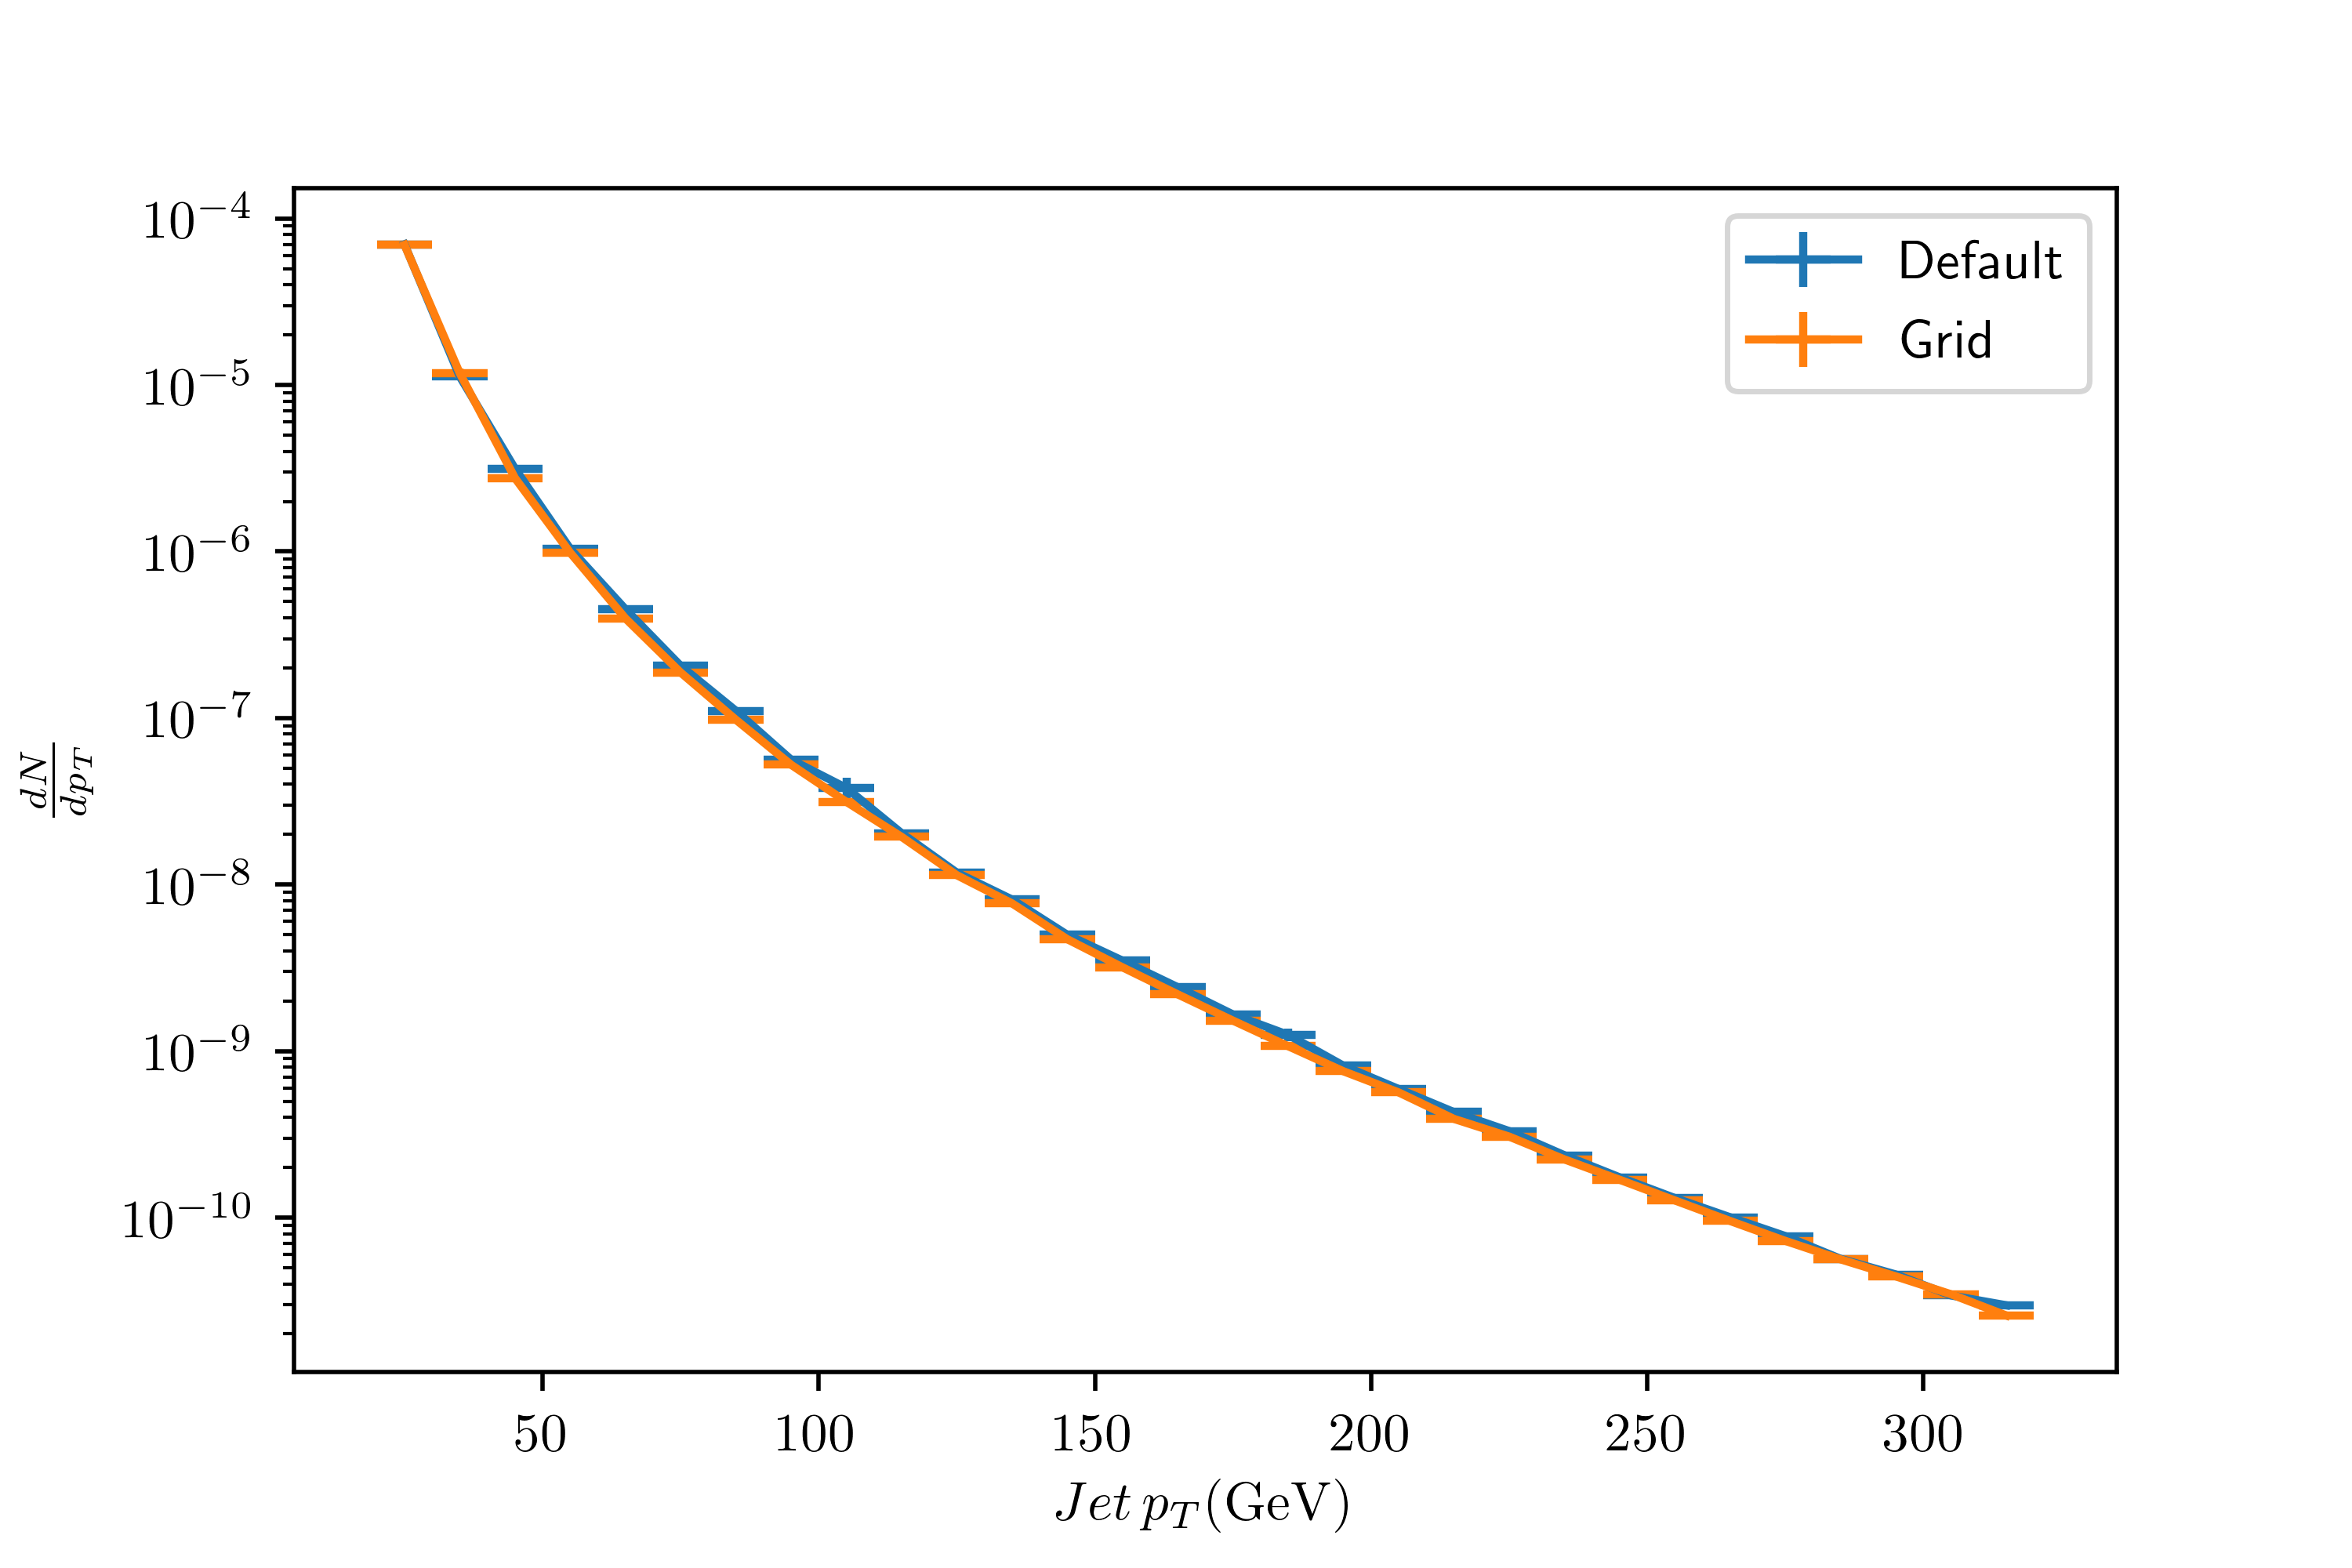
\includegraphics[width=0.7\textwidth]{images/grid_jetpt_validation.png}
\caption[Jet $p_T$ for Grid validation.]{Jet $p_T$ for Grid validation.}
\label{grid_jetpt_validation}
\end{figure}

\begin{figure}
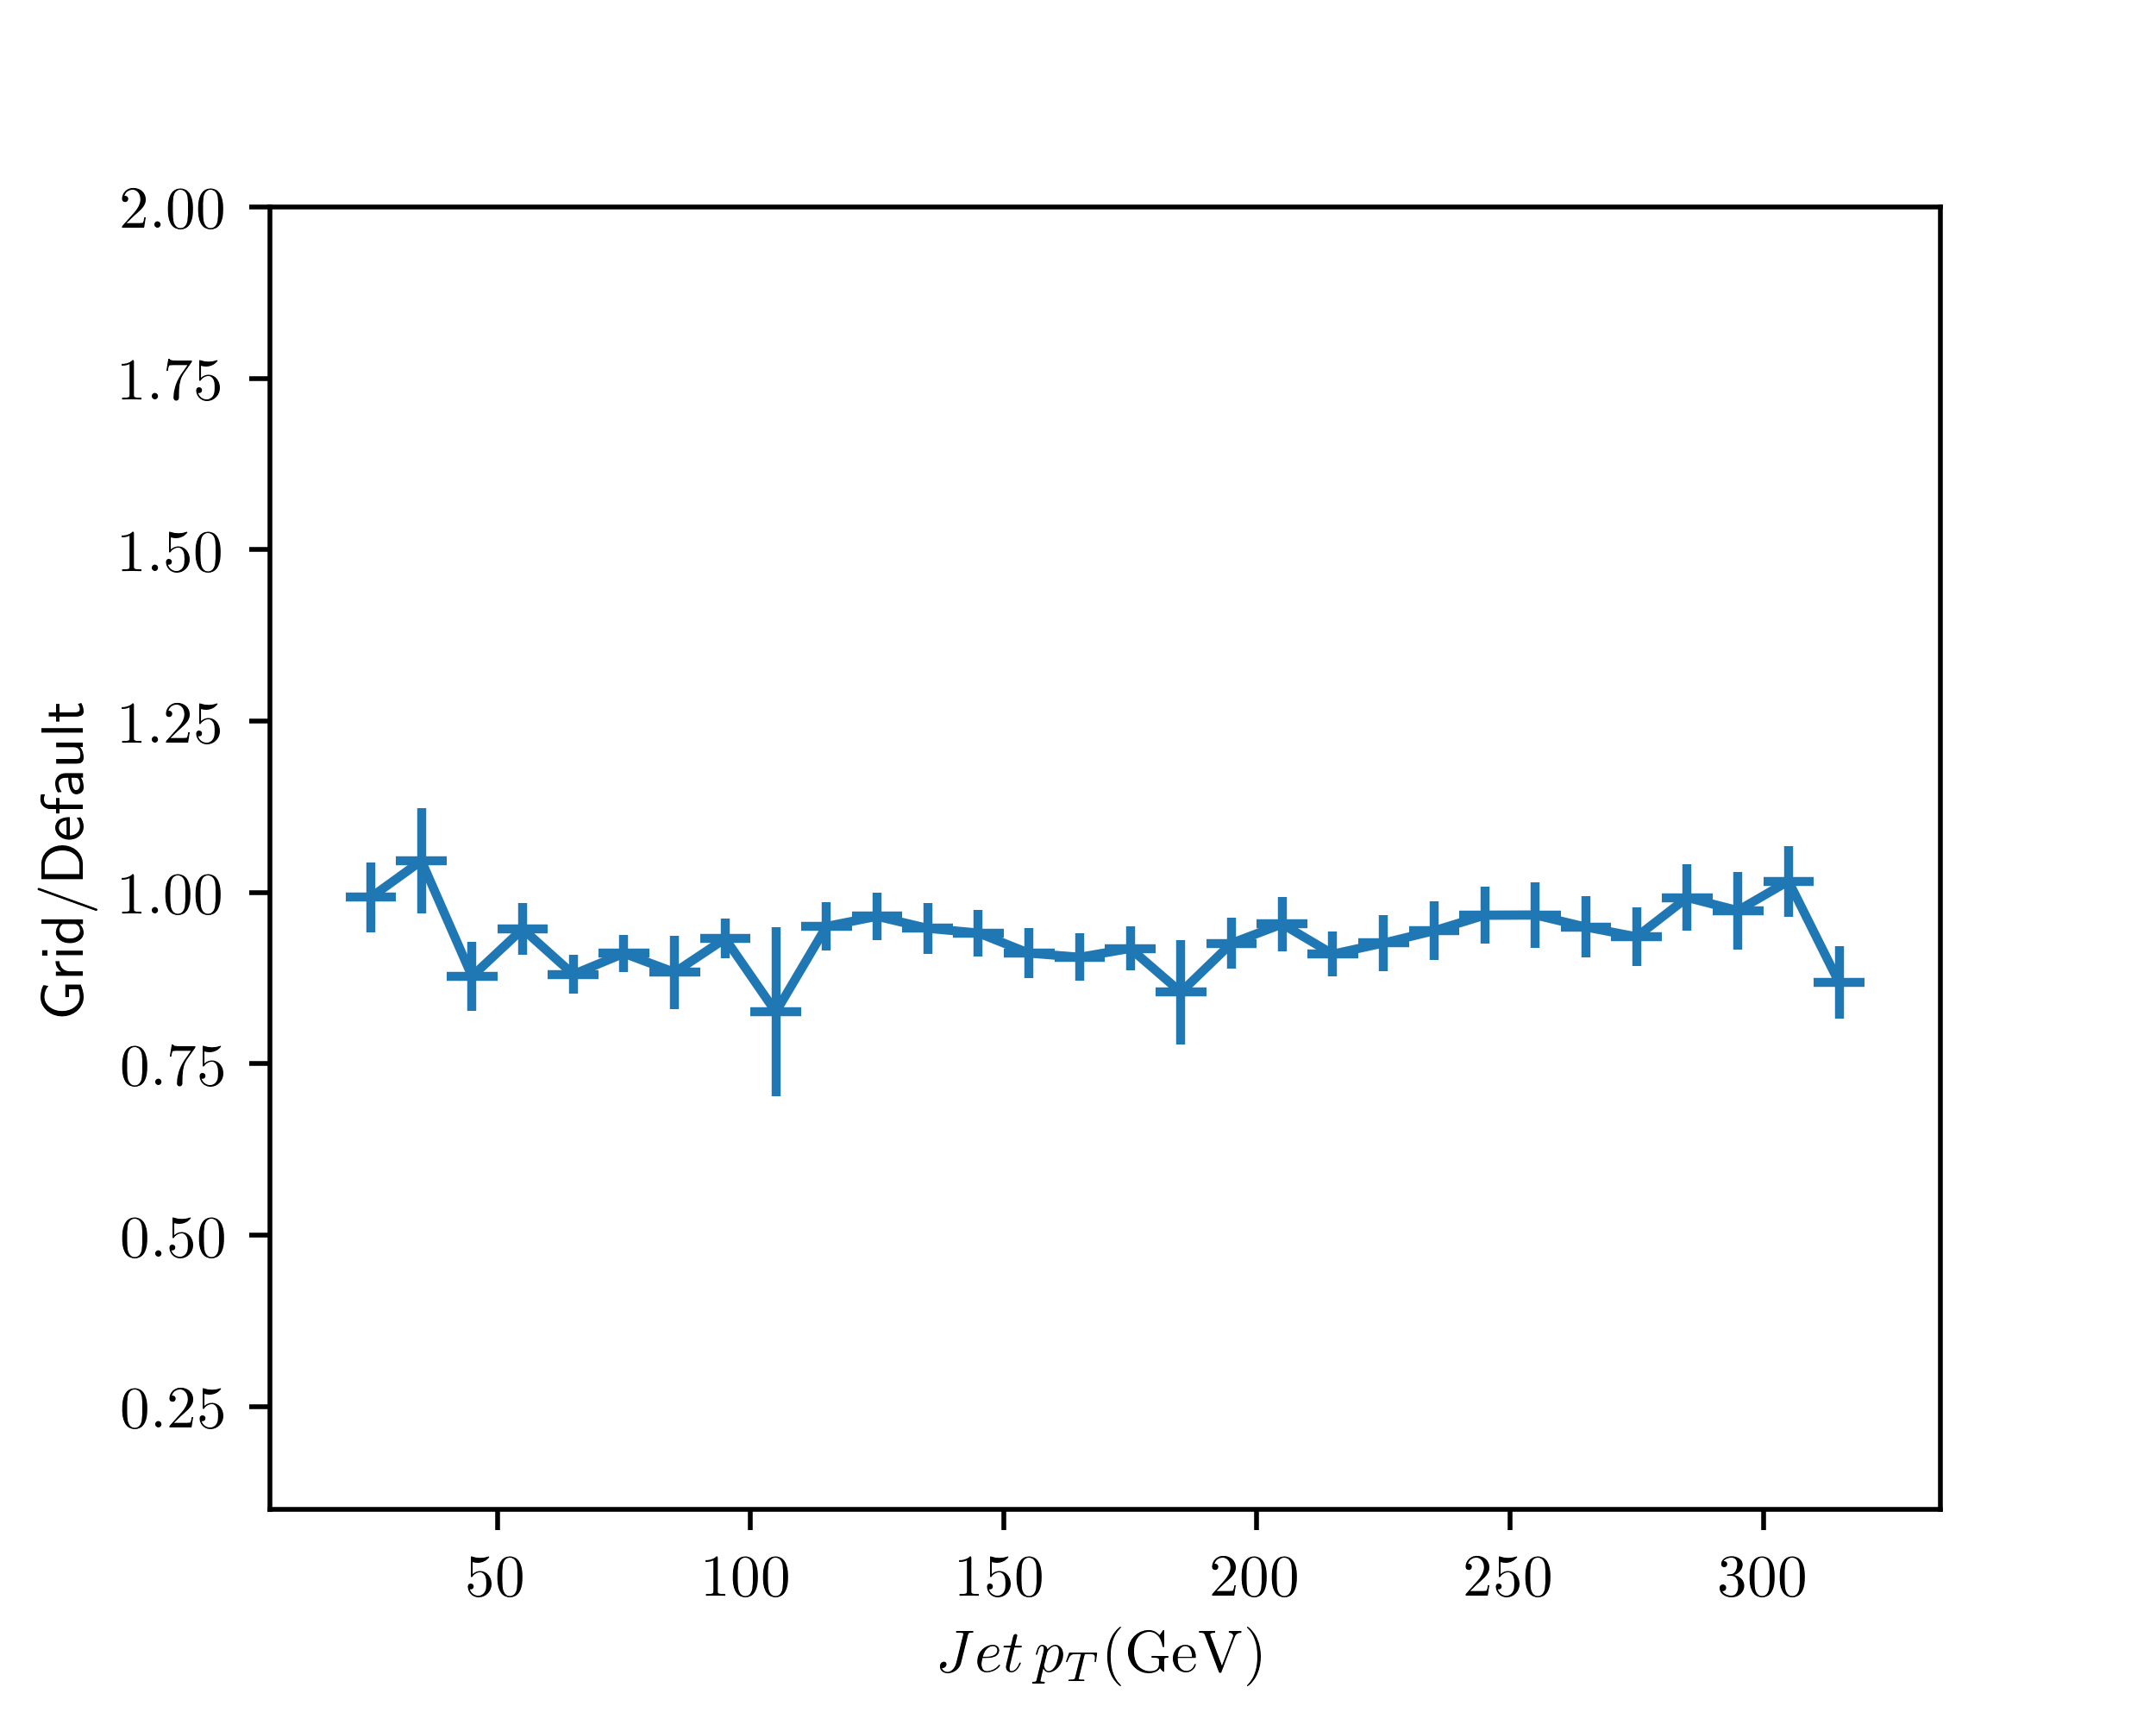
\includegraphics[width=0.7\textwidth]{images/grid_default_jetpt.png}
\caption[Grid/Default for jet $p_T$]{Grid/Default for jet $p_T$}
\label{grid_default}
\end{figure}

For the case jet mass we can see a plot of the spectra and a ratio plot on Figures \ref{grid_jetmass_validation} and \ref{grid_default_jetmass}, respectively. The mass has an error of $25\%$ in only one bin, but the rest of the bins is well controlled within the uncertainties. This shows that both methods agree. The peak and width of the distribution are well reproduced.

\begin{figure}
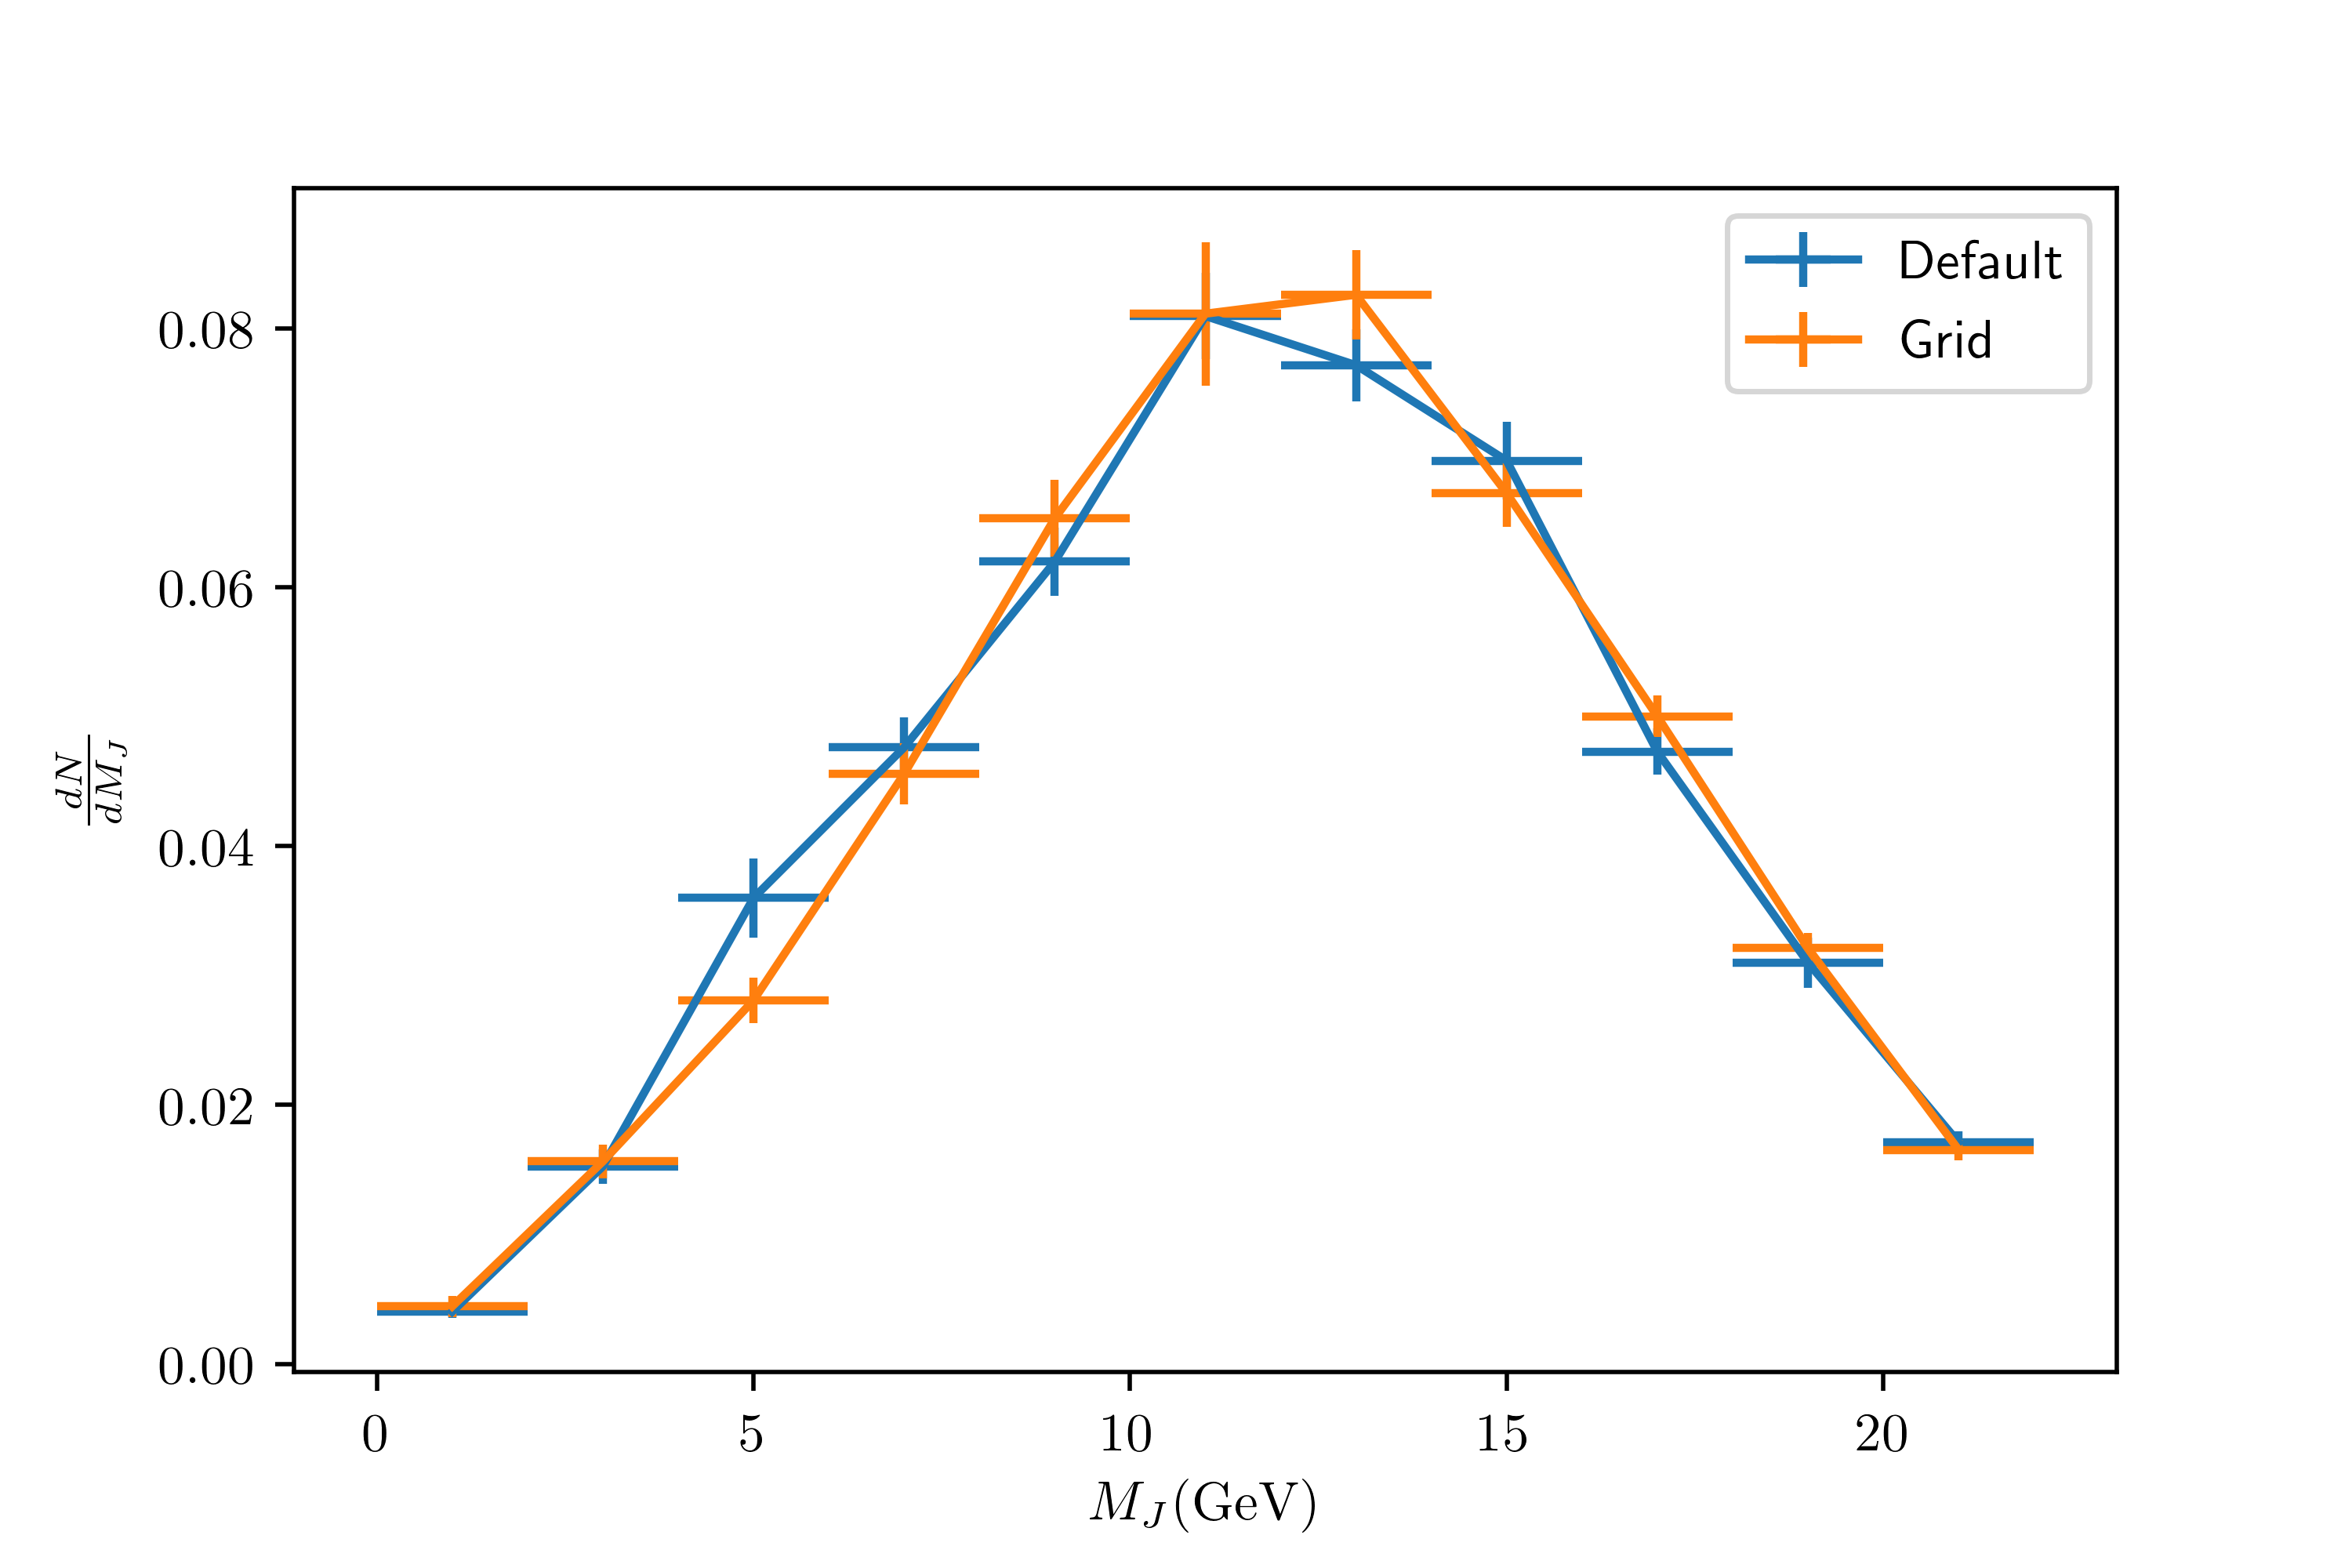
\includegraphics[width=0.7\textwidth]{images/grid_mass_validation.png}
\caption[Jet Mass for Grid validation.]{Jet Mass for Grid validation.}
\label{grid_jetmass_validation}
\end{figure}

\begin{figure}
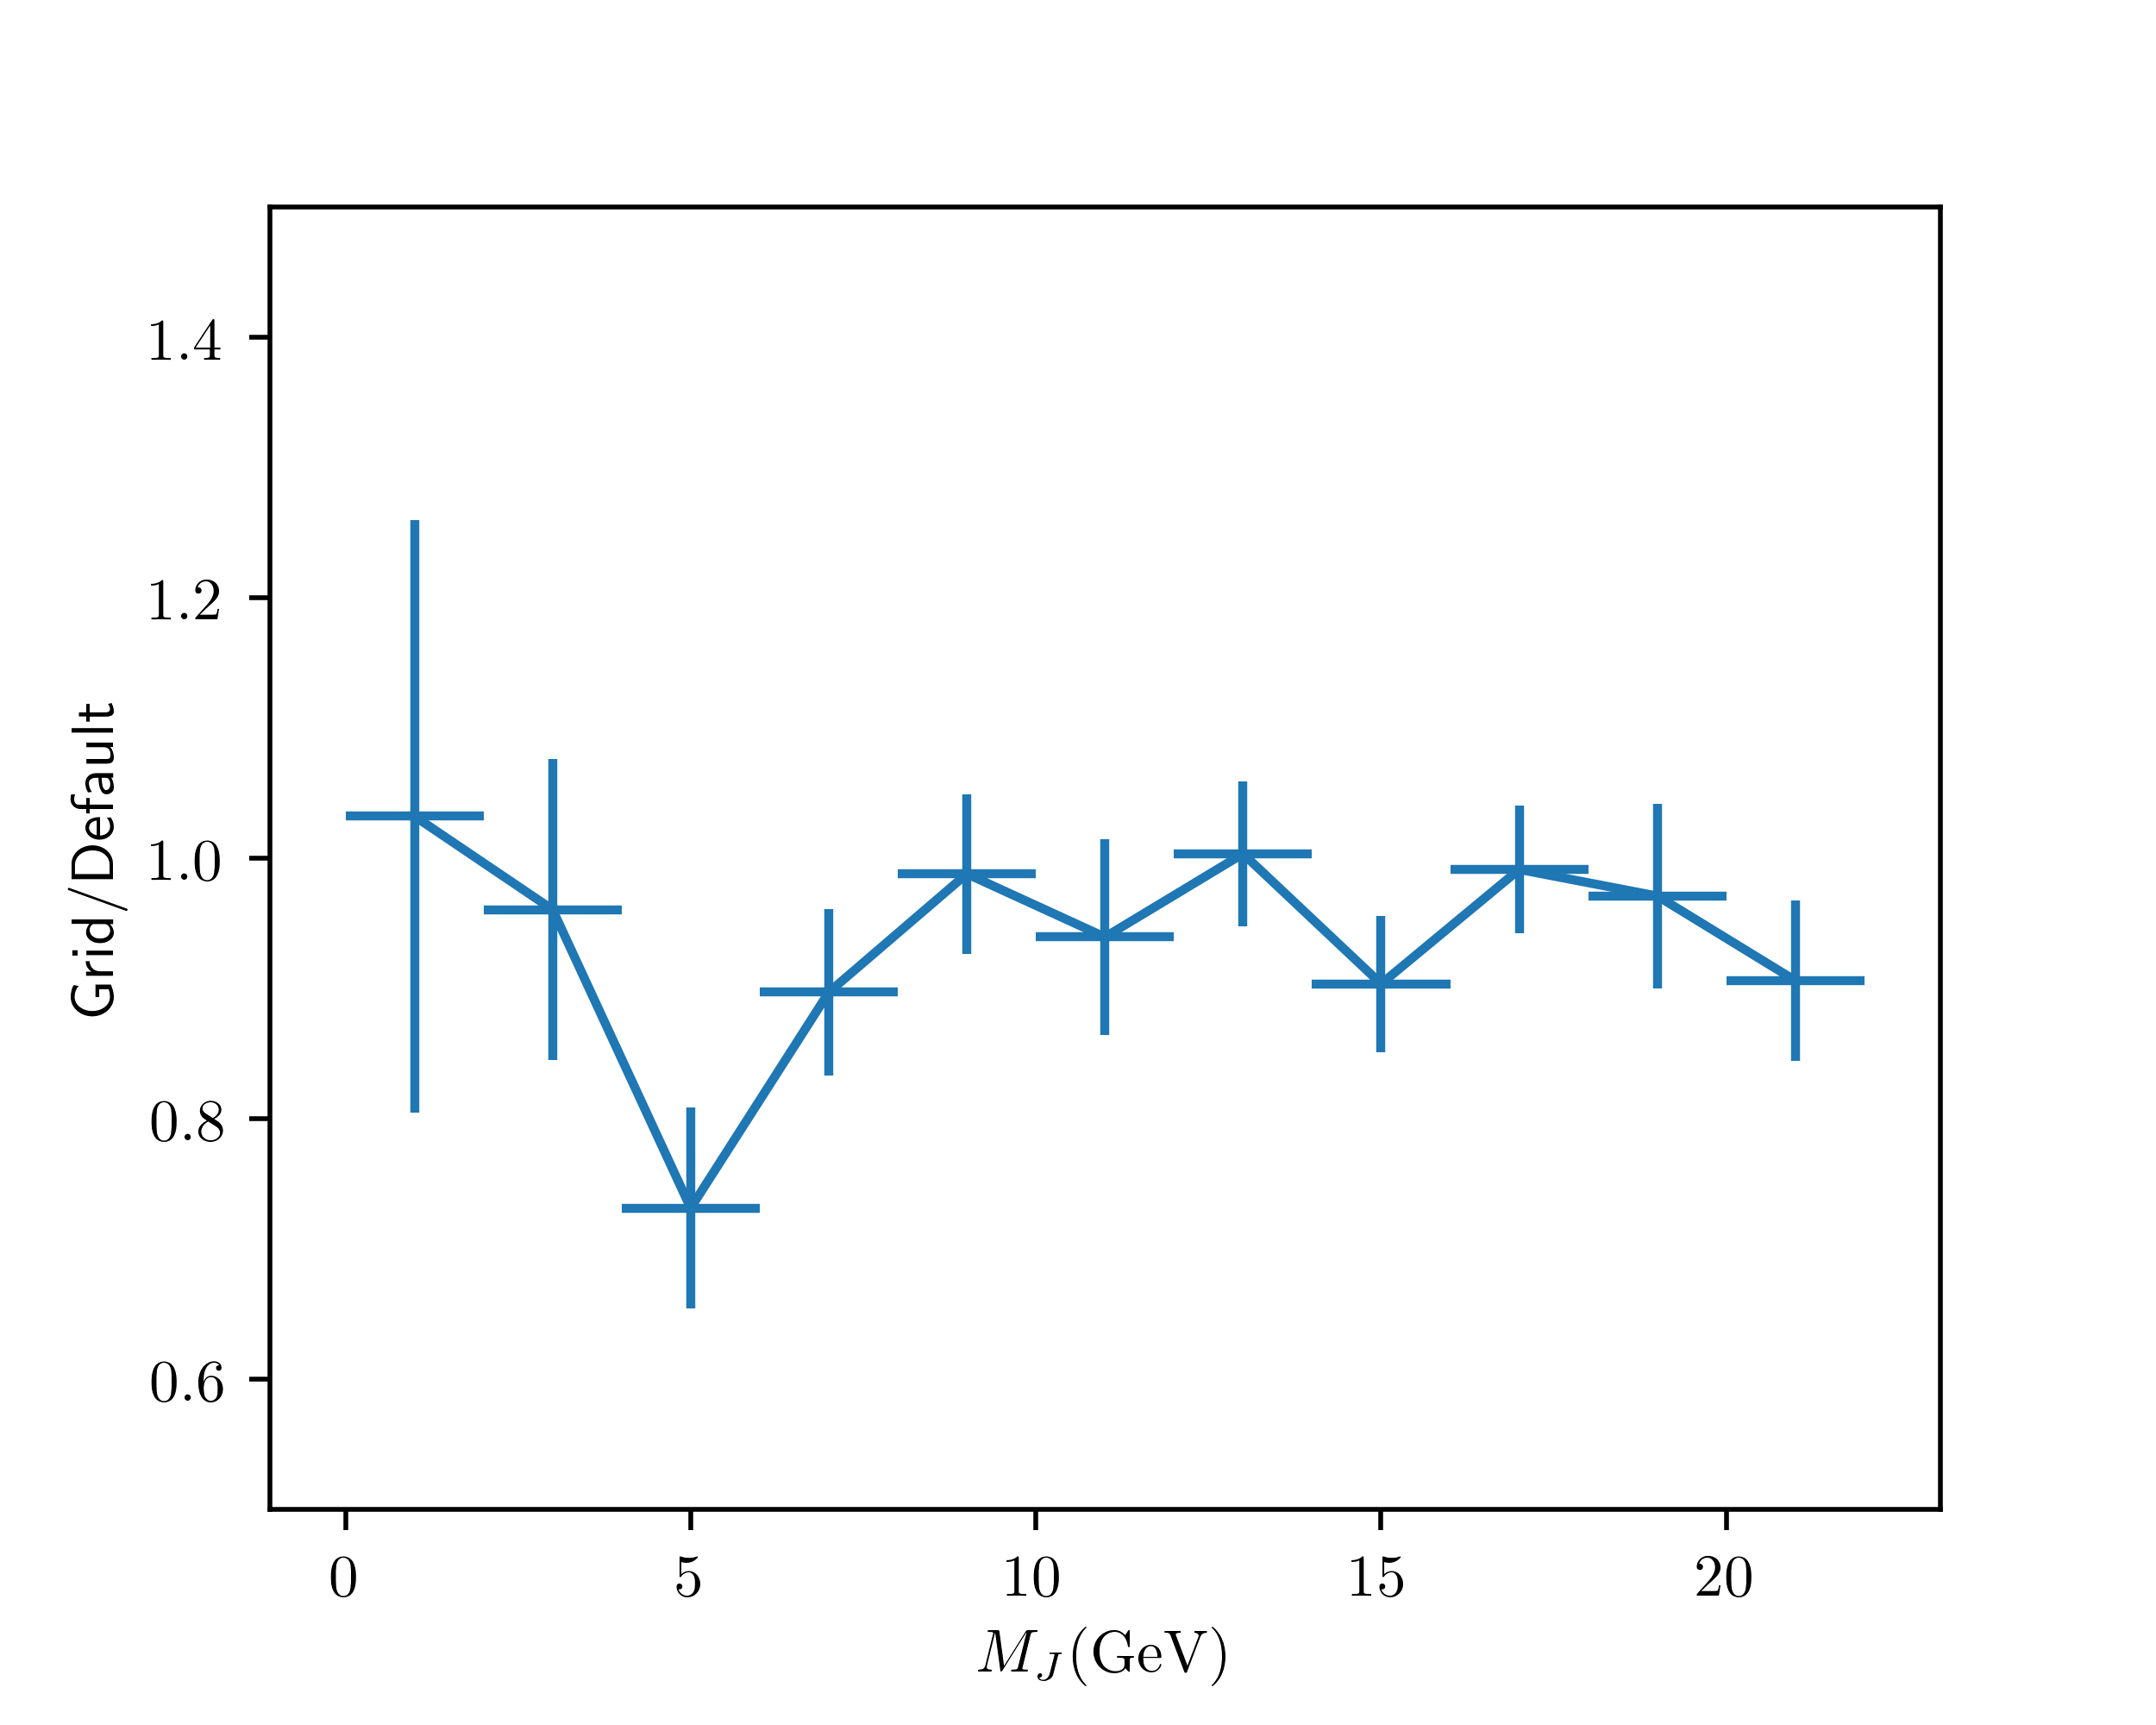
\includegraphics[width=0.7\textwidth]{images/grid_default_mass.png}
\caption[Grid/Default for jet mass]{Grid/Default for jet mass}
\label{grid_default_jetmass}
\end{figure}

On Figures \ref{grid_girth_validation} and \ref{grid_default_girth} we can see the plots for the jet girth for both cases and also a ratio plot. The qualitative behavior is reproduced. Within the uncertainties, the data of both methods agree. The peak and width of the distribution are well reproduced.

\begin{figure}
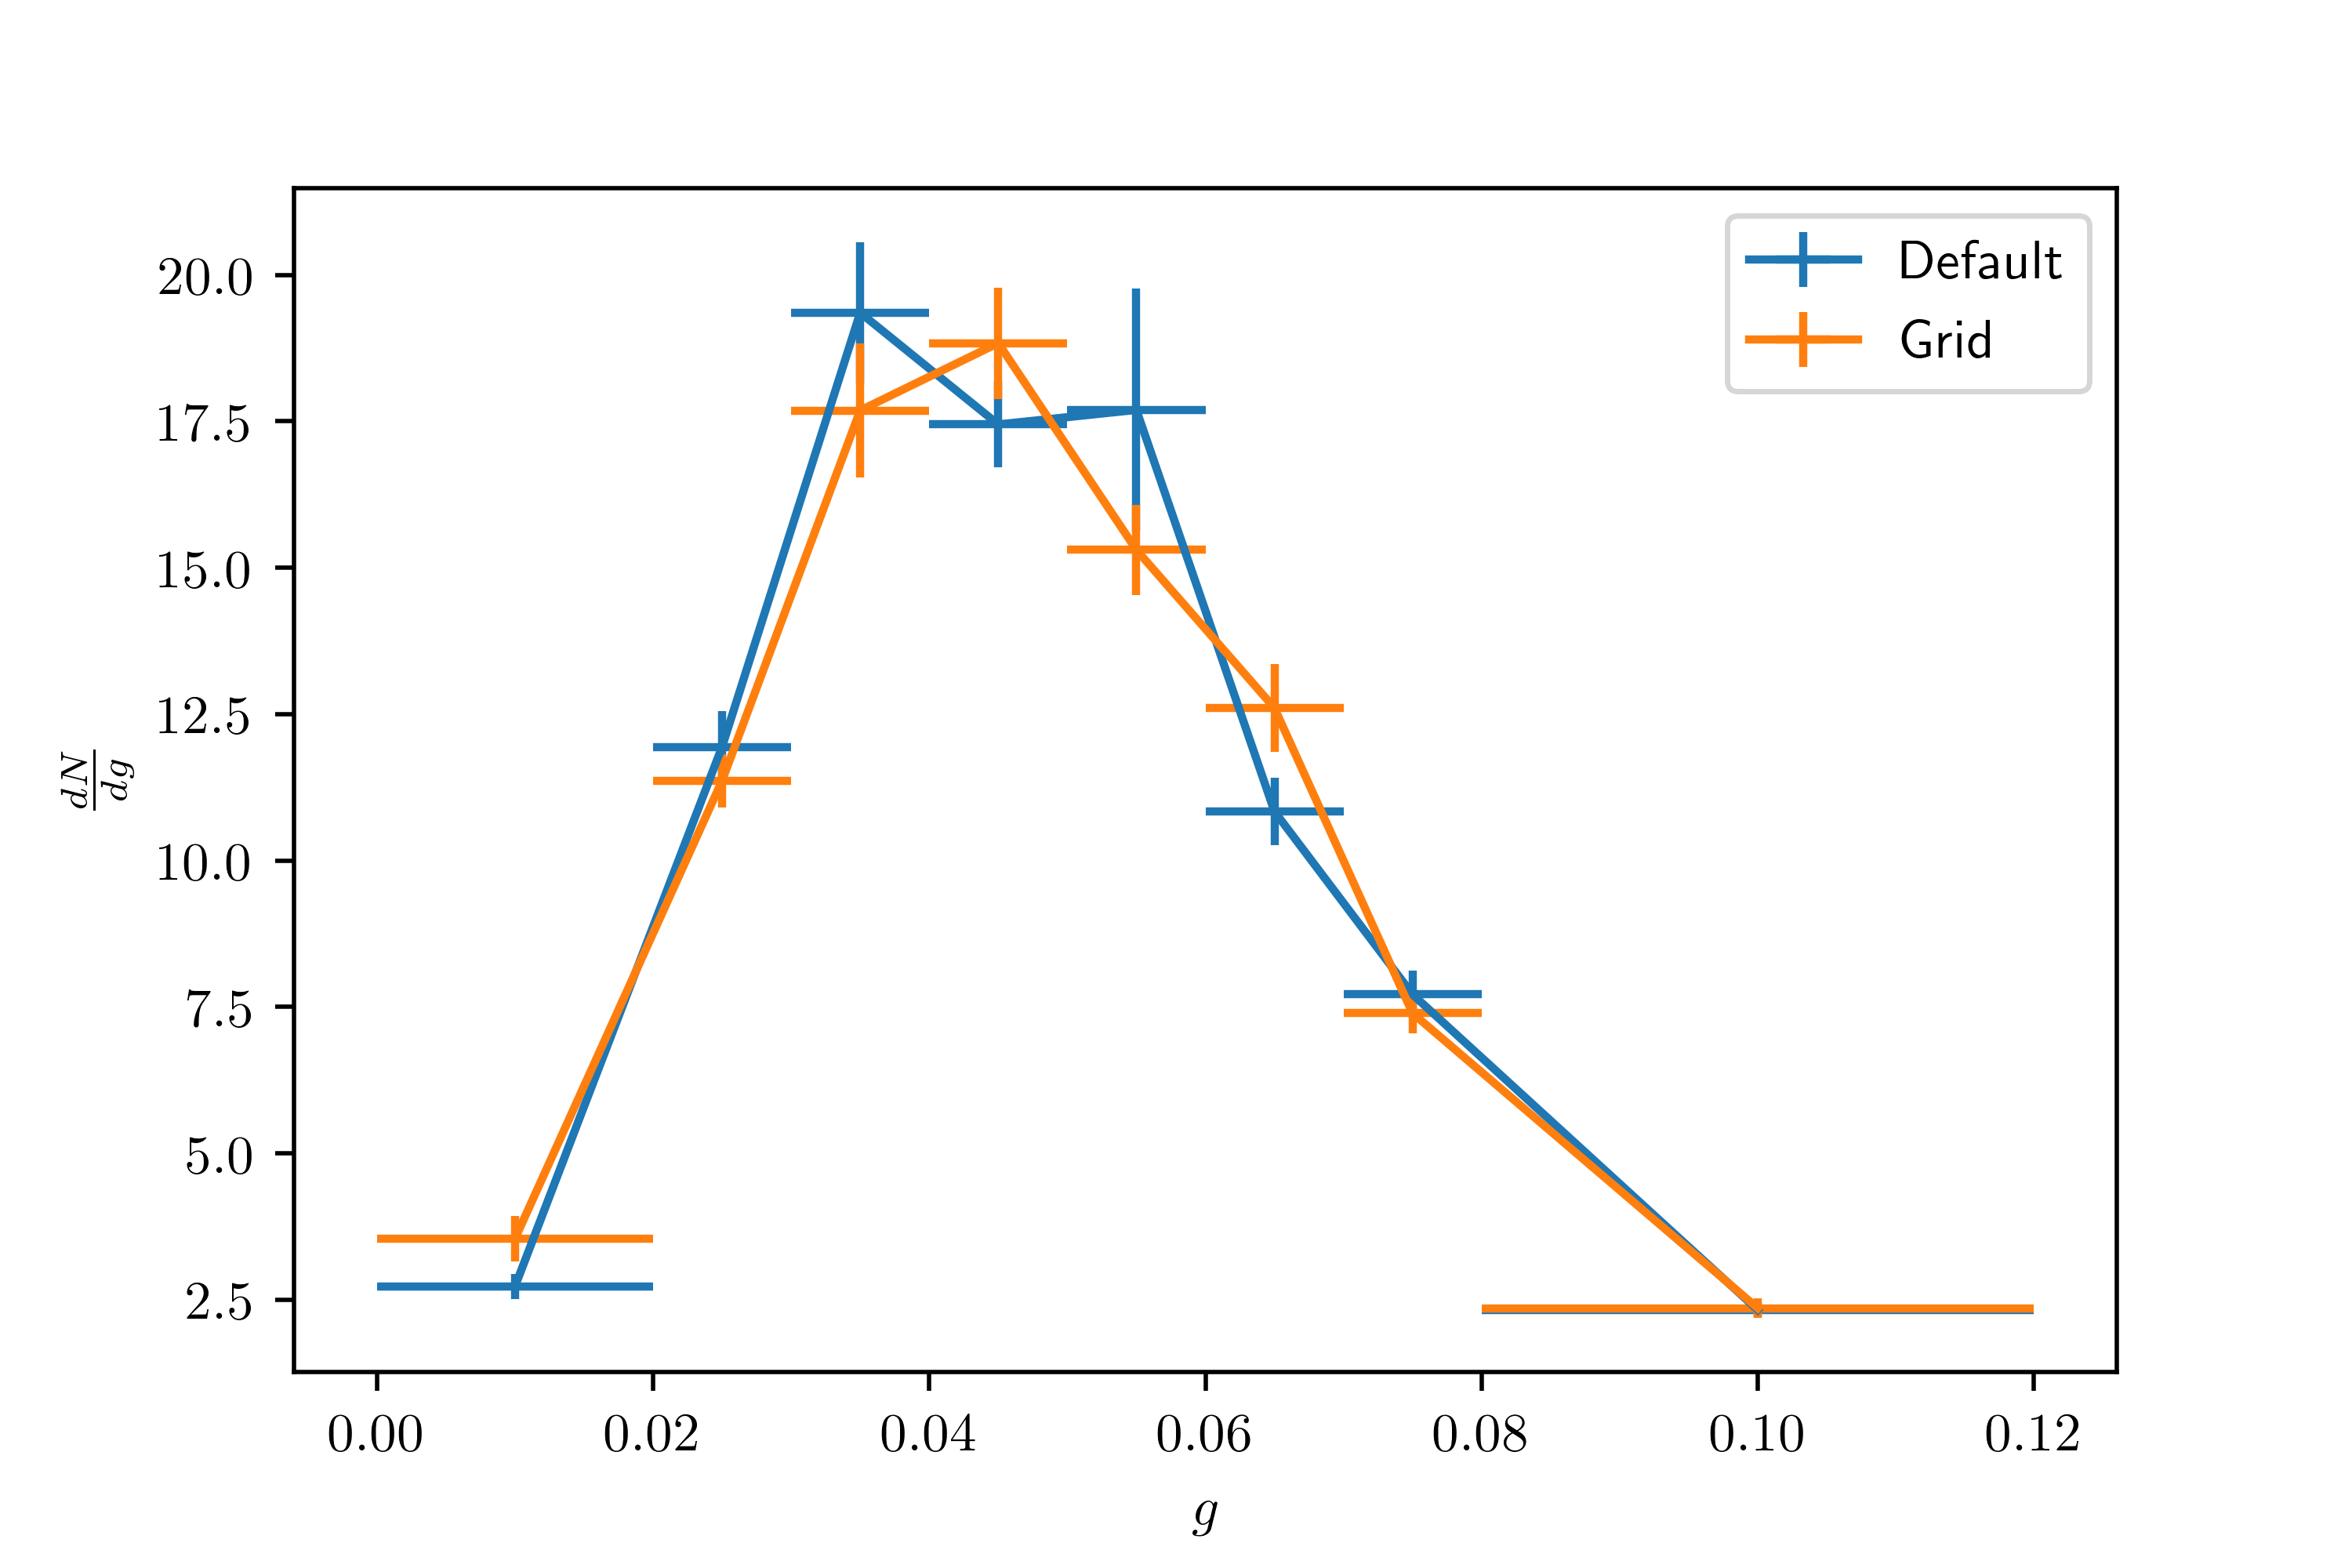
\includegraphics[width=0.7\textwidth]{images/grid_girth_validation.png}
\caption[Jet Girth for Grid validation.]{Jet Girth for Grid validation.}
\label{grid_girth_validation}
\end{figure}

\begin{figure}
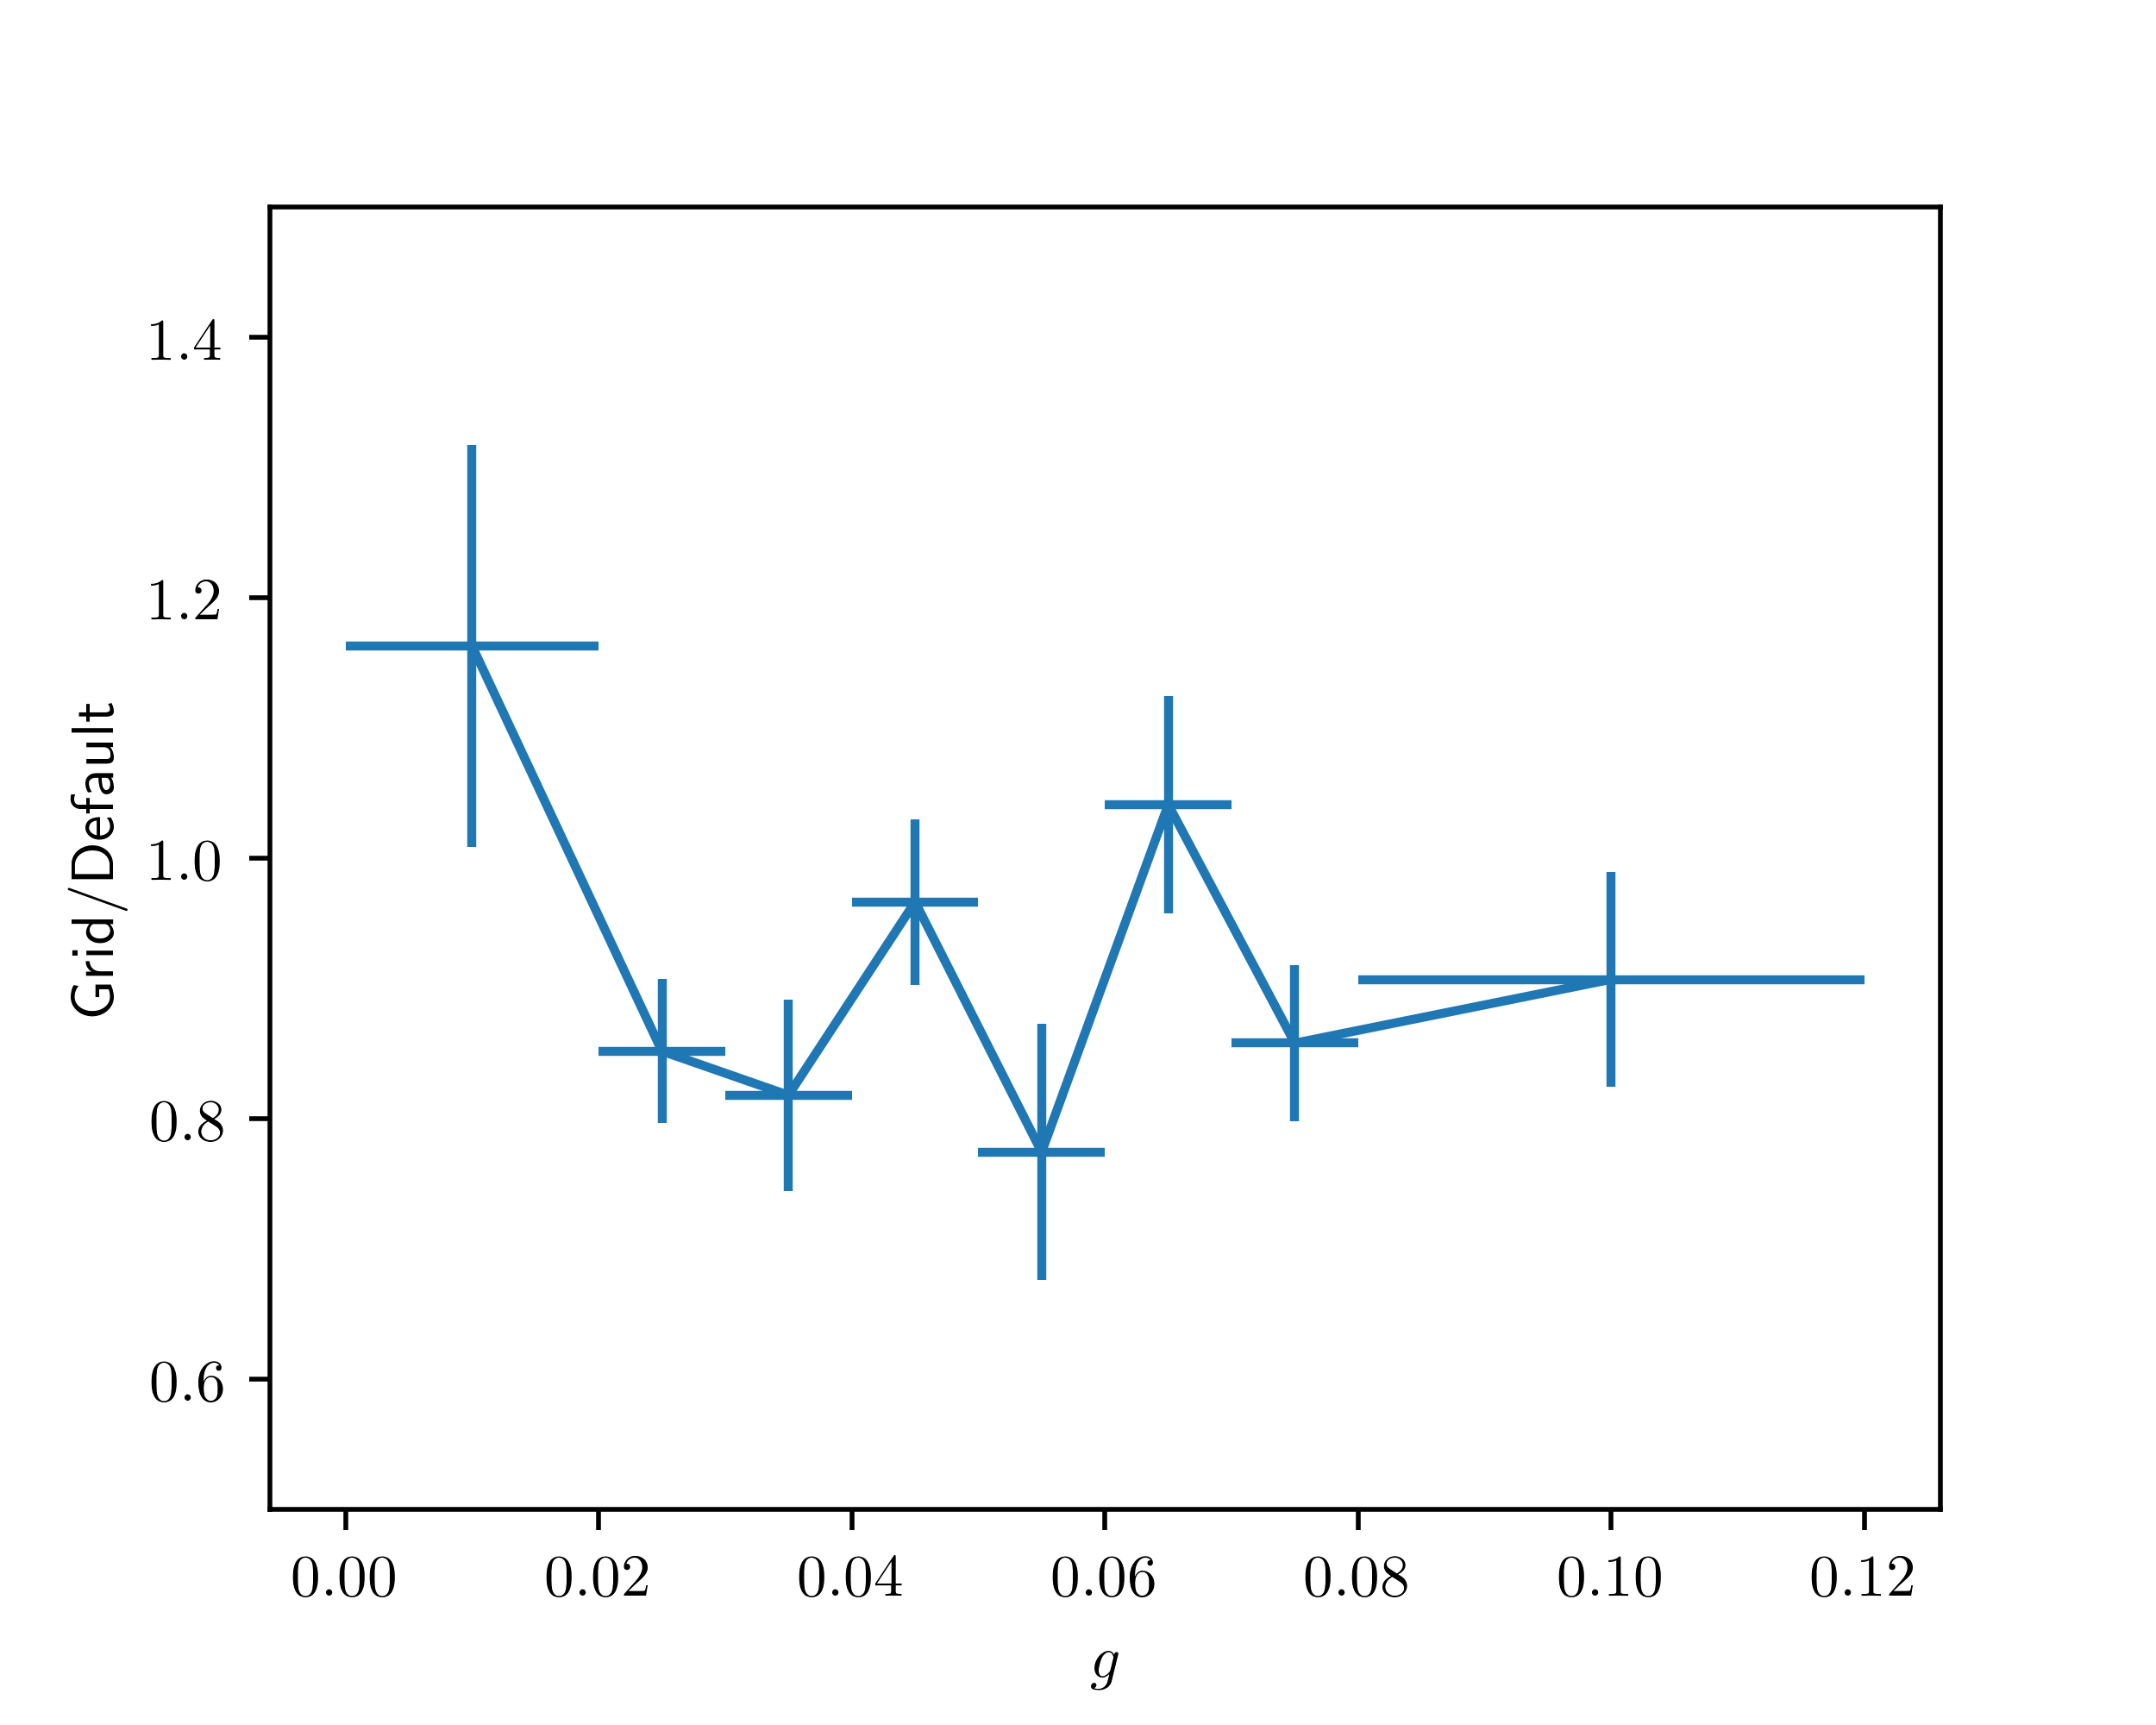
\includegraphics[width=0.7\textwidth]{images/grid_default_girth.png}
\caption[Grid/Default for jet girth]{Grid/Default for jet girth}
\label{grid_default_girth}
\end{figure}

On Figures \ref{grid_dispersion_validation} and \ref{grid_default_girth} we can see the plots for the jet $p_T^D$ for both cases and also a ratio plot. The qualitative behavior is reproduced. Within the uncertainties, the data of both methods agree. The peak and width of the distribution are well reproduced.

\begin{figure}
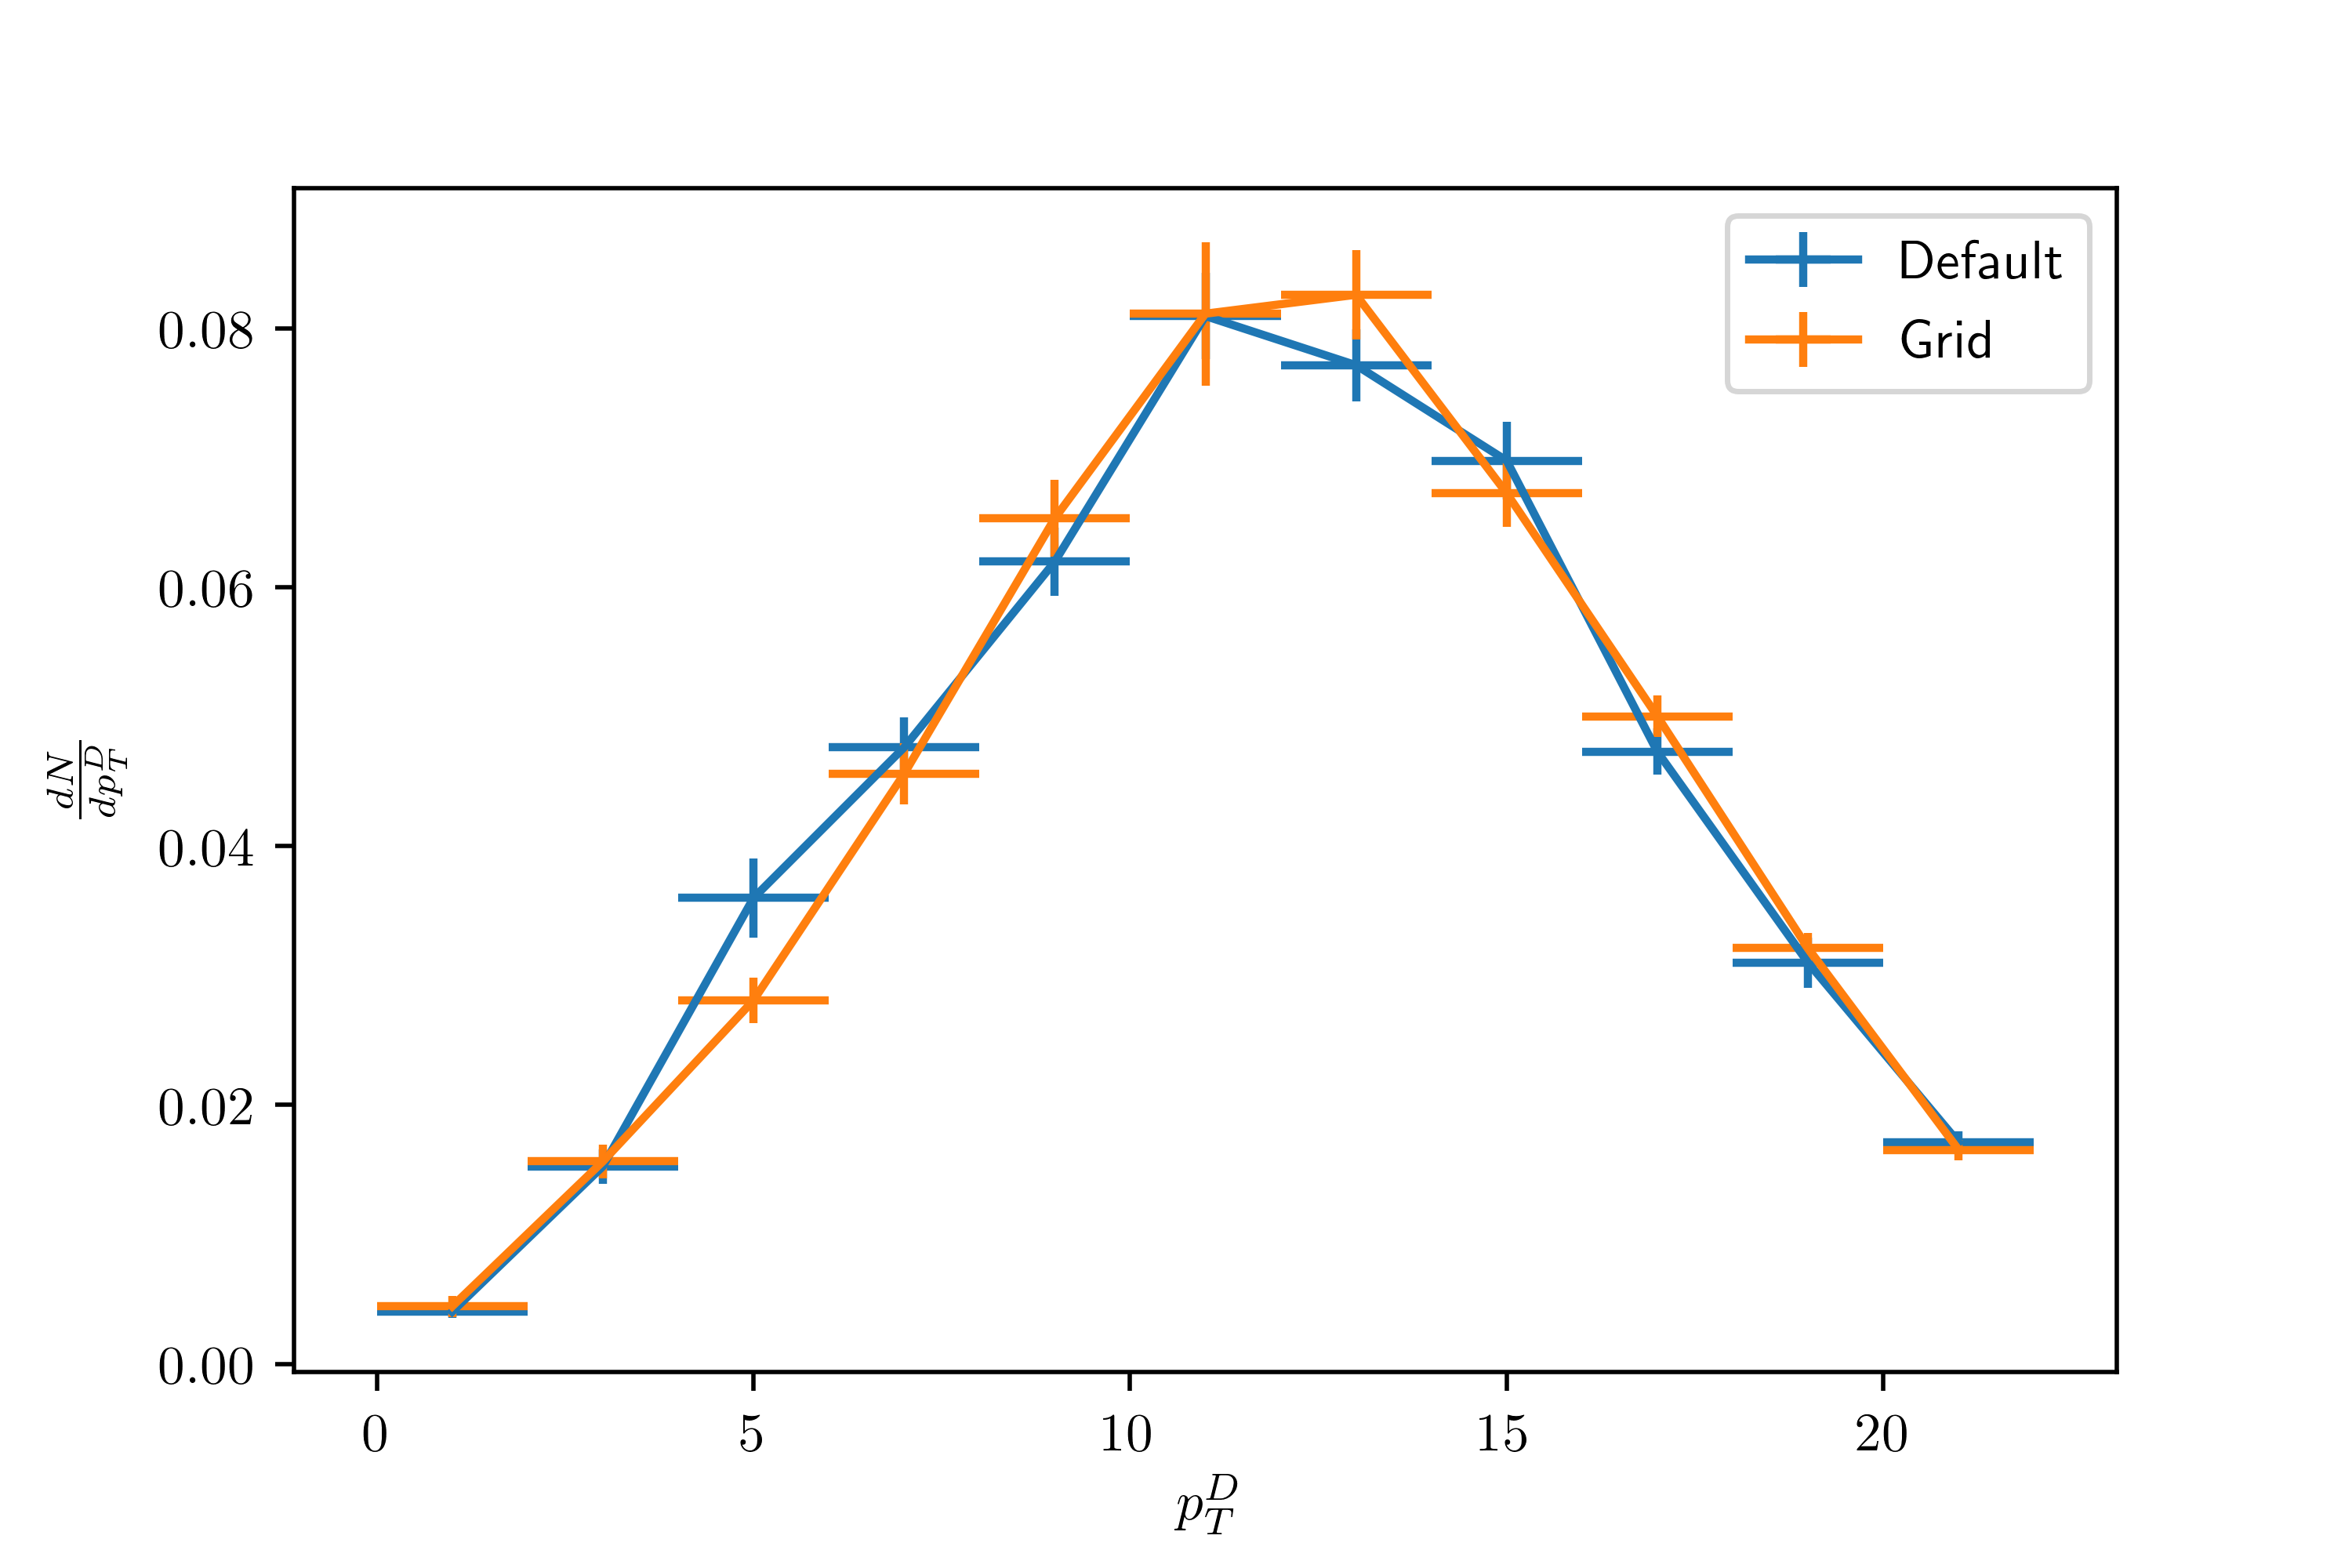
\includegraphics[width=0.7\textwidth]{images/grid_dispersion_validation.png}
\caption[Jet Dispersion for Grid validation.]{Jet Dispersion for Grid validation.}
\label{grid_dispersion_validation}
\end{figure}

\begin{figure}
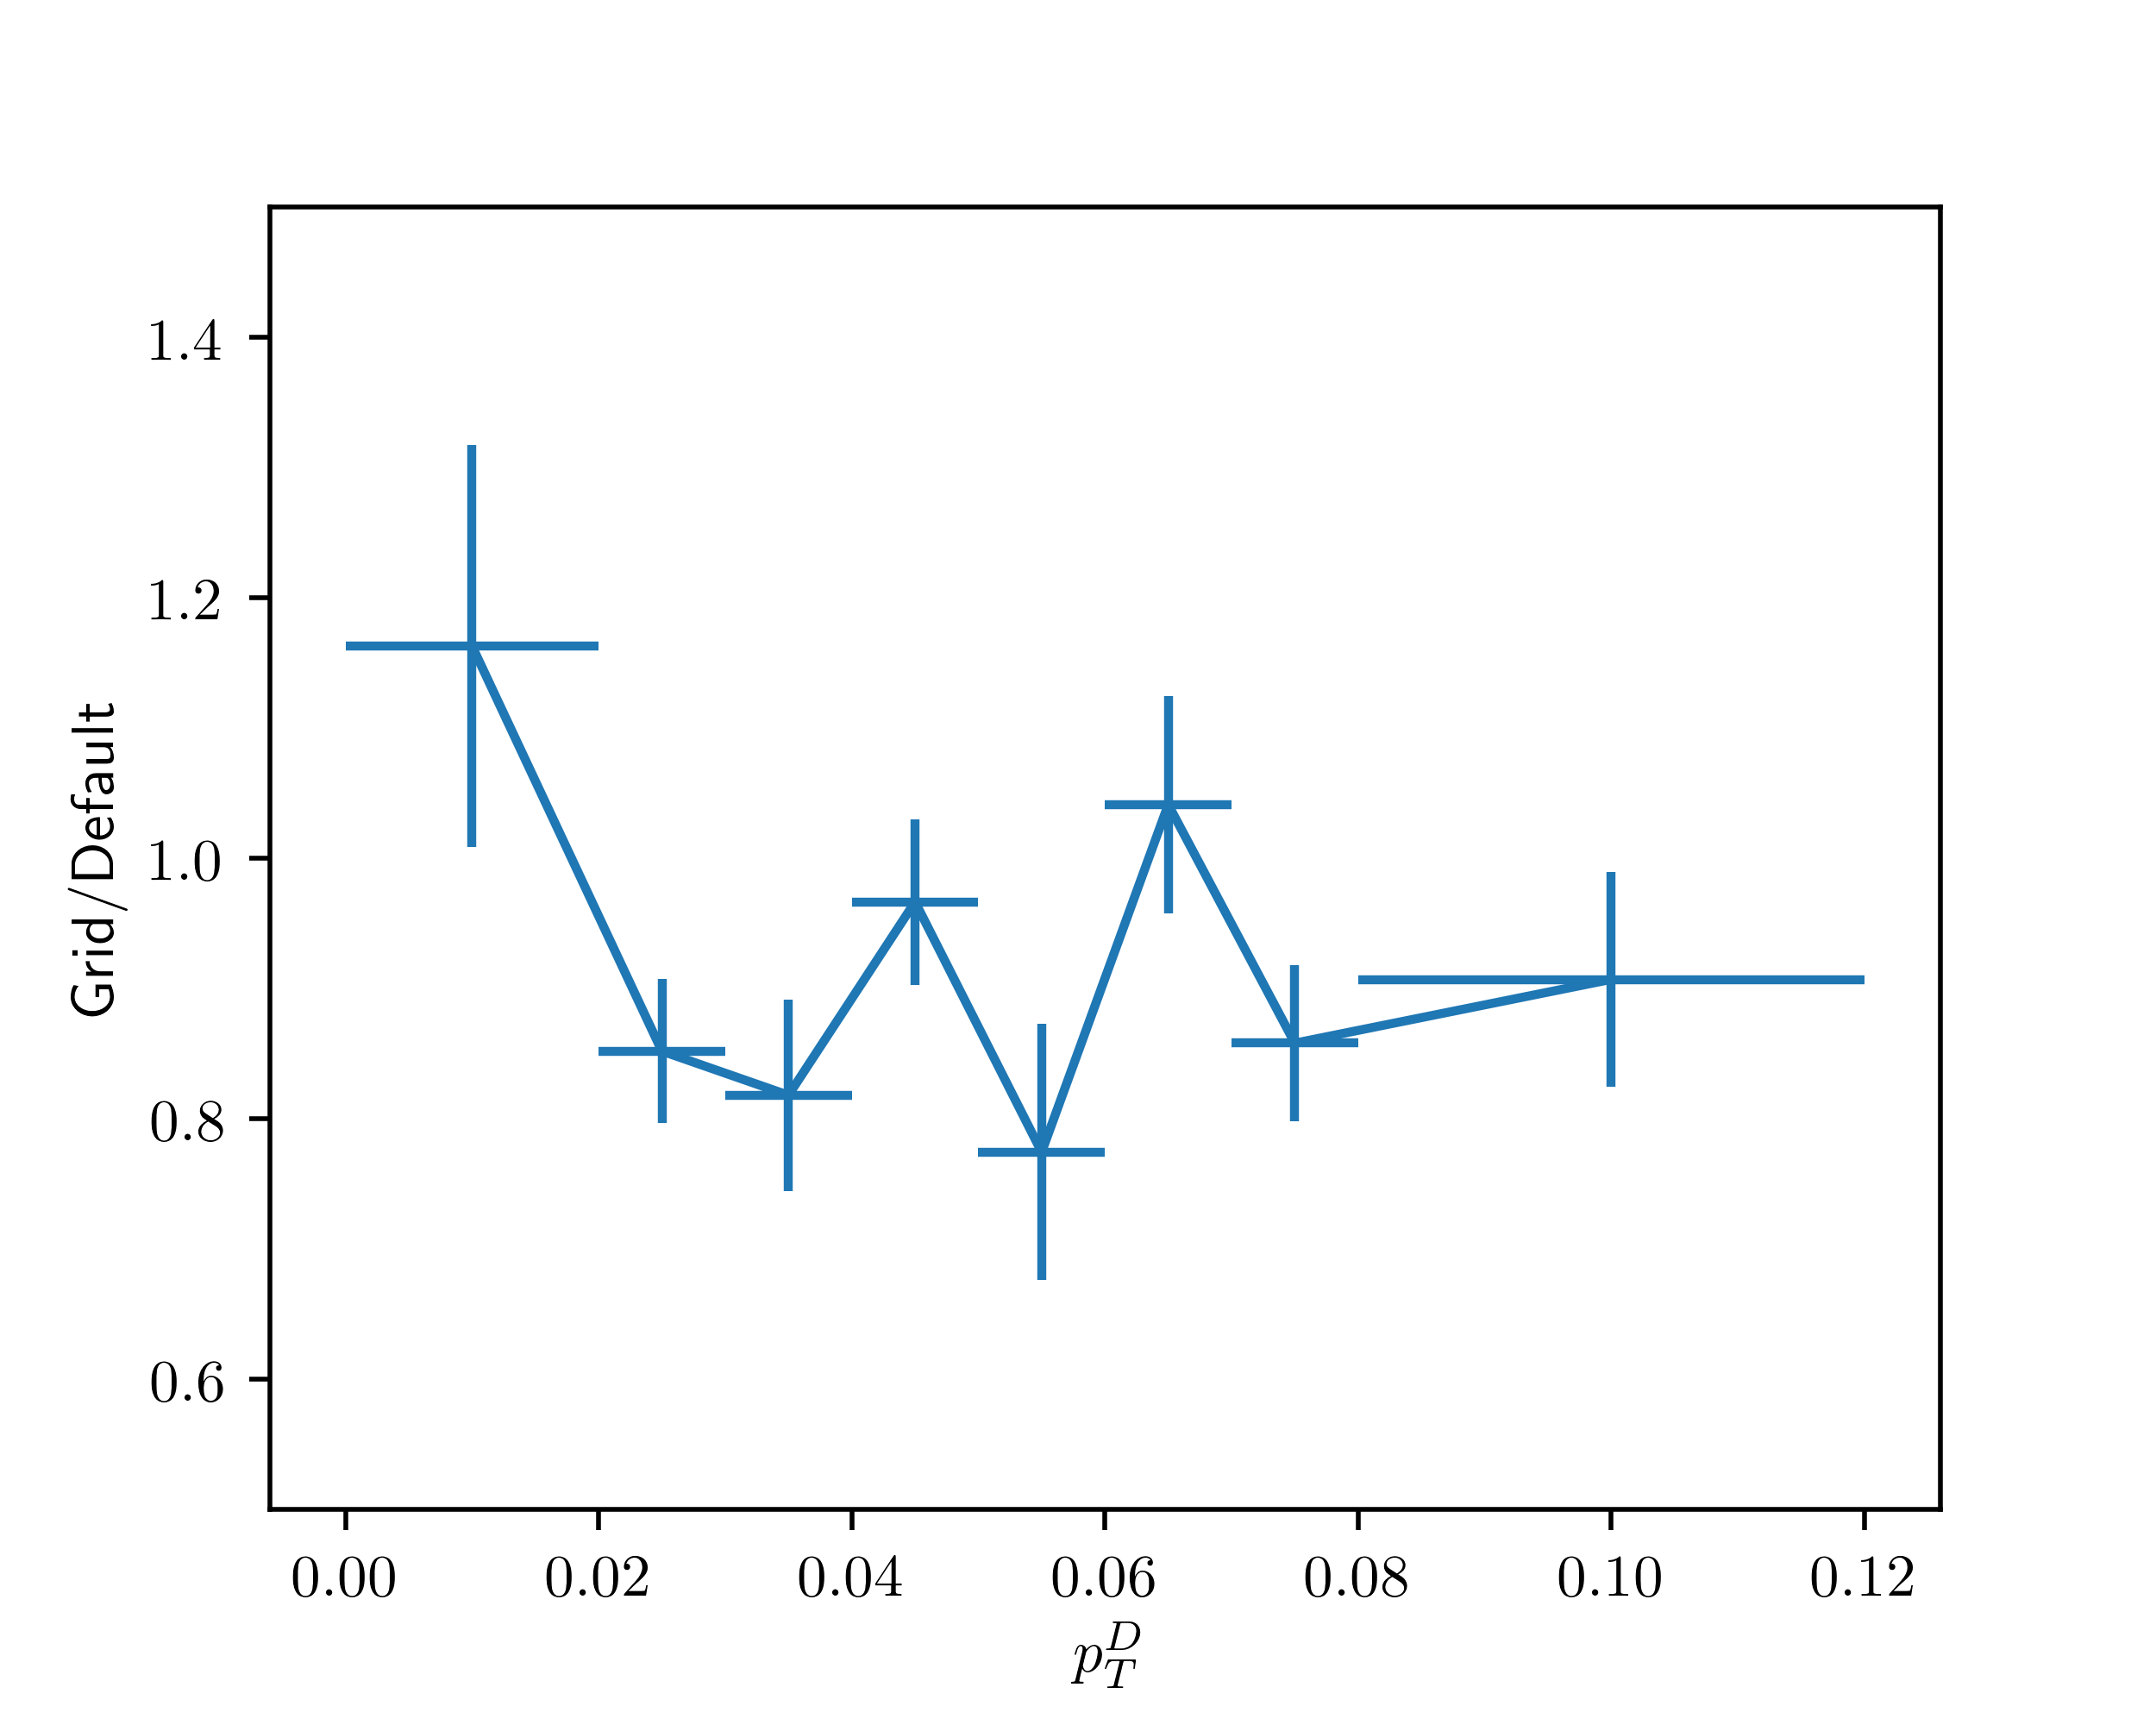
\includegraphics[width=0.7\textwidth]{images/grid_default_dispersion.png}
\caption[Grid/Default for jet dispersion]{Grid/Default for jet dispersion}
\label{grid_default_dispersion}
\end{figure}